\documentclass[11pt,a4paper]{report}

\usepackage[british]{babel}
\usepackage[none]{hyphenat} 
\usepackage{array}  % Put this in your preamble

% Define a new column type:
\newcolumntype{P}[1]{>{\raggedright\arraybackslash}p{#1}}

% Aberstwyth MMP Project Report Template for LaTeX
%
% Authors: Neil Taylor (nst@aber.ac.uk) and Dr. Hannah Dee (hmd1@aber.ac.uk) 
%
% This has been adapted from the Leeds Thesis template and the 
% Group Project template for Computer Science in Aberystywth University.
% 
% All comments and suggestions welcome.
%
% Template designed to be used with pdflatex: it may need alteration to
% run with a different LaTeX engine.
%
% Note - this is offered as a starting point for your work. You are not 
% required to use this template and can choose to create your own document 
% without it.

% This template is suitable for students with an engineering-style project, 
% which will be most students in the department. If your project is a research-oriented 
% project, look at the alternative template.

% To build document on the unix command line, run four commands:
 
% pdflatex mmp-report
% bibtex mmp-report
% pdflatex mmp-report
% pdflatex mmp-report

% you will end up with mmp-report.pdf. Before submitting, add your user ID as a prefix, 
% e.g. abc01-mmp-report.pdf 
\usepackage{StylesAndReferences/mmp-report}

% the following packages are used for citations - You only need to include one. 
%
% Use the cite package if you are using the numeric style (e.g. IEEEannot). 
% Use the natbib package if you are using the author-date style (e.g. authordate2annot). 
% Only use one of these and comment out or remove the other one. 
\usepackage{cite}
%\usepackage{natbib}

%Package used to embed PDF into report
%Source - https://www.pdfconverters.net/how-to/insert-pdf-to-latex/
\usepackage{pdfpages}

%Packages used to list code in a reasonable and colour-coded format
%Source - https://www.overleaf.com/learn/latex/Code_Highlighting_with_minted
\usepackage{minted}
\usepackage{listings}
\usepackage{color}

% **TODO**
%Source - https://tex.stackexchange.com/questions/166743/automatic-line-break-in-tabular
\usepackage{tabularx}
\usepackage{longtable}

% Source - https://tex.stackexchange.com/questions/2441/how-to-add-a-forced-line-break-inside-a-table-cell
\usepackage{makecell}

%Package used to include Braket (Dirac) Notation
\usepackage{braket}

% Source - https://tex.stackexchange.com/questions/204621/matrix-in-latex
\usepackage{amsmath}

% Source - https://tex.stackexchange.com/questions/73160/table-with-tabularx-and-multirow
\usepackage{multirow}

% Source - https://www.overleaf.com/learn/latex/Questions/How_can_I_write_a_%C2%B0_(degree)_symbol_in_LaTeX%3F
\usepackage{gensymb}

% Source - https://tex.stackexchange.com/questions/43008/absolute-value-symbols
\usepackage{commath}

% Source - https://tex.stackexchange.com/questions/156016/how-do-i-make-a-small-pmatrix
\usepackage{mathtools}
\newenvironment{brsm}{% % short for 'bracketed small matrix'
  \bigl[ \begin{smallmatrix} }{%
  \end{smallmatrix} \bigr]}

% Source - https://tex.stackexchange.com/questions/1774/how-to-insert-pipe-symbol-in-latex
\usepackage[T1]{fontenc}

% Source - https://tex.stackexchange.com/questions/157389/how-to-center-column-values-in-a-table
\usepackage{array}
\newcolumntype{P}[1]{>{\centering\arraybackslash}p{#1}}
\newcolumntype{M}[1]{>{\centering\arraybackslash}m{#1}}

% Source - https://tex.stackexchange.com/questions/485794/reduce-padding-in-cell-with-lists-in-tabularx/
\usepackage{enumitem}
\newlist{tabitemize}{itemize}{1}
\setlist[tabitemize]{nosep,
                  topsep= 0pt,
                  partopsep=0pt,
                  leftmargin= *,
                  label=\textbullet,
                  before=\vspace{-0.6\baselineskip},
                  after=\vspace{-\baselineskip}
                  }

\usepackage{pgfplots}

\usepackage{microtype}
\usepackage{graphicx}
\usepackage{pdflscape}

\usepackage[nottoc]{tocbibind} 

\usepackage{tocloft}    % for list of equations
\usepackage{ragged2e}   % to undo \centering
\usepackage{hyperref}   % to make references hyperlinks
\usepackage{glossaries} 

%\usepackage[hidelinks]{hyperref}
\usepackage[nameinlink]{cleveref}

\crefname{figure}{Figure}{Figures}
\Crefname{figure}{Figure}{Figures}

\crefname{table}{Table}{Tables}
\Crefname{table}{Table}{Tables}

\crefname{equation}{Equation}{Equations}
\Crefname{equation}{Equation}{Equations}

\crefname{chapter}{Chapter}{Chapters}
\Crefname{chapter}{Chapter}{Chapters}

\crefname{section}{Section}{Sections}
\Crefname{section}{Section}{Sections}

\crefname{appendix}{Appendix}{Appendices}
\Crefname{appendix}{Appendix}{Appendices}

% List of Equations
\newcommand{\listequationsname}{List of Equations}
\newlistof{myequations}{equ}{\listequationsname}

\newcommand{\myequation}[1]{%
    \addcontentsline{equ}{myequations}{%
        \protect\numberline{\theequation}#1%
    }%
}

\setlength{\cftmyequationsindent}{1.5em}
\setlength{\cftmyequationsnumwidth}{2.3em}

% Source - https://tex.stackexchange.com/questions/37420/is-it-possible-to-count-text-in-tables-using-texcount
%TC:group table 1 1 

%%%% Title and Section Colours %%%%
% Modify these values to change the colours used for title, sections and subsections.
% Each value is a range of 0-255 in RGB colourspace.
% Idea courtesy of discussion at 
% https://www.overleaf.com/learn/latex/Using_colours_in_LaTeX
% and
% https://tex.stackexchange.com/questions/75667/change-colour-on-chapter-section-headings-lyx
% 
% If you prefer to have black headers, then comment out the following lines
\definecolor{mmpTitle}{RGB}{255, 128, 000}
\definecolor{mmpSection}{RGB}{255,128,000}
\definecolor{mmpSubsection}{RGB}{083,086,090}

\chapterfont{\color{mmpTitle}}  % sets colour of chapters
\sectionfont{\color{mmpSection}}  % sets colour of sections 
\subsectionfont{\color{mmpSubsection}} % sets colour subsections
\subsubsectionfont{\color{mmpSubsection}} % sets colour subsections

%%%% end of Title and Section Colours %%%%
\renewcommand{\listequationsname}{{\color{mmpTitle}\Huge\bfseries List of Equations}}
\renewcommand{\cfttoctitlefont}{\color{mmpTitle}\Huge\bfseries}
\renewcommand{\cftloftitlefont}{\color{mmpTitle}\Huge\bfseries}
\renewcommand{\cftlottitlefont}{\color{mmpTitle}\Huge\bfseries}
%\renewcommand{\cftmyequationstitlefont}{\color{mmpTitle}\Huge\bfseries}



%%%% Report Type %%%%
%% comment/uncomment depending on the type of report you want to generate
\reporttype{Engineering}
%\reporttype{Research}
%%%% end of Report Type %%%%


\begin{document}

%TC:ignore

% all of the include directives below refer to tex files
% so \include{cover} includes cover.tex - to change the content,
% edit the tex file

\pagenumbering{roman}

% This is the front page
%TC:ignore 

\title{Undercut Analysis from Historic Lap Time Data in Formula One}

% Your name
\author{Harry Adams}

% Your email 
\authoremail{harry.adams@mclaren.com}

%\degreeschemecode{G401} %e.g. G400 
\degreeschemetitle{Advanced Motorsport Engineering} % e.g. Computer Science
\degreetype{MSc}

\modulecode{Module 9 - } % i.e. CS39440, CC39440, CS39620
\moduletitle{Advanced Motorsport Project - } % i.e. Major Project or Minor Project

\date{\today} % i.e. the date of the current version of your report

\status{Draft} % Use draft until you create the release version. Then, change this to Release.
\version{0.1}

% The title and name of your supervisor.
\supervisor{Tim Mullis} 

%The email for your supervisor. 
\supervisoremail{tim@motorsport.nda.ac.uk}

\maketitle

%TC:endignore
                        

% Set up page numbering
\pagestyle{empty}

% declarations of originality 
\thispagestyle{empty}

%TC:ignore

%%%
%%% You must sign the declaration of originality. 
%%%
%%% You are submitting this electronically. Therefore, to sign, you 
%%% type your name and date to replace the .... characters. 
%%%
\section*{\centering Declaration of originality}

I confirm that:

\begin{itemize}
\item{This submission is my own work, except where 
clearly indicated.}

\item{I understand that there are severe penalties for Unacceptable Academic Practice, which can lead to loss of marks or even the withholding of a degree.}
 
\item{I have read the regulations on Unacceptable Academic Practice from the University's Academic Registry (AR) and the relevant sections of the current Student Handbook.}
 
\item{In submitting this work I understand and agree to abide by the University's regulations governing these issues.}
\end{itemize}

\vspace{2em}
Name: Harry Adams  \\

\vspace{1em}
Date: TODO \\

%%% 
%%% We would like to make a selection of final reports available to students that take 
%%% this module in future years. To enable us to do this, we require your consent. You 
%%% are not required that you do this, but if you do give your consent, then we will have 
%%% the option to select yours as one of a number of reports as examples for other 
%%% students. If you would like to give your consent, then please include the following 
%%% text and type your name and date to replace the .... characters. 
%%% 
%%% If you do not wish to give your consent, please remove this from your report. 
%%%
\vspace{1em}
\section*{\centering Consent to share this work}

By including my name below, I hereby agree to this project's report and technical work being made available to other students and academic staff of the National Motorsport Academy.  

\vspace{2em}
Name: Harry Adams  \\

\vspace{1em}
Date: TODO \\

%TC:endignore

               

\thispagestyle{empty}

%TC:ignore

\section*{\centering Acknowledgements}

Lorem Ipsum

%TC:endignore % Acknowledgements

\thispagestyle{empty}

%TC:ignore

\section*{\centering Abstract}

Lorem Ipsum


%TC:endignore                 % Abstract

\pagenumbering{roman}
\pagestyle{fancy}
\fancyhead{}
\fancyfoot[C]{\thepage}
\renewcommand{\headrulewidth}{0 pt}
\renewcommand{\chaptermark}[1]{\markboth{#1}{}}


% Set up page numbering
\pagenumbering{arabic}

\tableofcontents
\newpage

\listoffigures
\newpage

\listoftables
\newpage

\addcontentsline{toc}{chapter}{List of Equations}
\listofmyequations
\newpage

\chapter*{List of Abbreviations}
\addcontentsline{toc}{chapter}{List of Abbreviations}

\begin{center}
\begin{tabular}{p{0.7\textwidth}p{0.2\textwidth}}
\textbf{Full Term} & \textbf{Abbreviation} \\ \hline
\textit{Fédération Internationale de l'Automobile} & FIA \\
\end{tabular}
\end{center}
\chapter*{List of Units}
\addcontentsline{toc}{chapter}{List of Units}

\begin{center}
\begin{tabular}{p{0.7\textwidth}p{0.2\textwidth}}
\textbf{Unit Name} & \textbf{Symbol} \\ \hline
Kilometres & km \\
Seconds & s \\
Degrees Celcius & {\degree}C \\
\end{tabular}
\end{center}

\setchapterheaderfooter


%TC:endignore

% include the chapters
\chapter{Background and Research Context}
\label{chap:background}

% ============================================================================
% CHAPTER PURPOSE -- HIGH PRIORITY
% Establish the motorsport and academic context required to understand the
% undercut problem. The reader should finish this chapter understanding:
%   1. why pit stop timing matters in modern Formula One;
%   2. how tyre behaviour creates an undercut opportunity;
%   3. what stay out, undercut and overcut strategies mean in race terms;
%   4. what relevant work already exists; and
%   5. the specific gap addressed by this project.
%
% Keep equations, model variables and software design out of this chapter.
% Those belong in Chapters \ref{chap:model} and \ref{chap:implementation}.
% ============================================================================

\section{Formula One Race Strategy}
\label{sec:race-strategy-background}

% HIGH PRIORITY -- approximately 0.5--1 page.
% Explain only the history needed to reach the modern tyre-strategy problem:
% - early emphasis on reliability, fuel and mechanical preservation;
% - refuelling as a strategic variable;
% - the 2010 refuelling ban and increased significance of tyre timing;
% - modern strategic decisions under mandatory tyre-compound rules.
% Cite regulations and authoritative motorsport/strategy sources.
% Avoid a broad history of F1 that does not support the research problem.

Since the beginning of the Formula One World Championship (F1) in 1950, races have been won and lost through a combination of vehicle performance, driver performance and strategic decision-making. The relative influence of each factor has changed as the technical and sporting regulations have evolved.

Early pit stops were frequent and done out of mechanical necessity. Cars were less fuel efficient and did not have tanks which could hold a race's worth of fuel, especially given that races were initially raced at ~500 kilometres rather than the maximum 320km set in 1971 \cite{F1Technical2009RaceDistance} and still used today. They were uncoordinated and dangerous affairs; fuel poured in from jerry cans risking dangerous blowback \cite{MotorSport1994Refuelling}, central wheel nuts secured with hammers \cite{Driver612022WheelNuts}, and upwards of a minute stationary while the mechanics worked. The time lost typically meant that race strategy was of minimal concern as it was heavily outweighed by practicalities.

Strategic pit stop strategies still occurred but were also far more simplistic, typically only considering the extra weight of fuel and newer tyres. The earliest example of the "tactical" pit stop is considered to be Juan Manuel Fangio in the 1957 German Grand Prix, who pitted on lap eleven and emerged fifty one seconds behind two Ferraris, before repeatedly setting fastest laps of the race and breaking the circuit records, before overtaking both cars on the final lap to secure his fifth World Championship, and his twenty fourth and final race win \cite{RaceFans2008PitStops}. This would be expanded into what more closely resembles a modern pit stop, with dedicated engineered equipment and tactical consideration, by Brabham at the 1982 Austrian Grand Prix who arrived with "what looked like beer kegs, huge diameter hoses, a blue chimney and a system to power the wheel guns" \cite{Automobilist2024PitStopRevolution}. The kegs were pressurised fuel delivery systems, capable of pumping 130 litres of fuel in three seconds, while the blue chimney was the predecessor to tyre blankets, with a gas blower heater at the bottom and small windows to check temperatures. Patrese's car would not finish the race, but it had demonstrated the effectiveness of pit stop equipment and influenced various regulations, such as the banning of refuelling from 1984-1994 \cite{FIA1984TechnicalRegulations} and from 2010 \cite{FIA2010SportingRegulations}. 

\begin{figure}
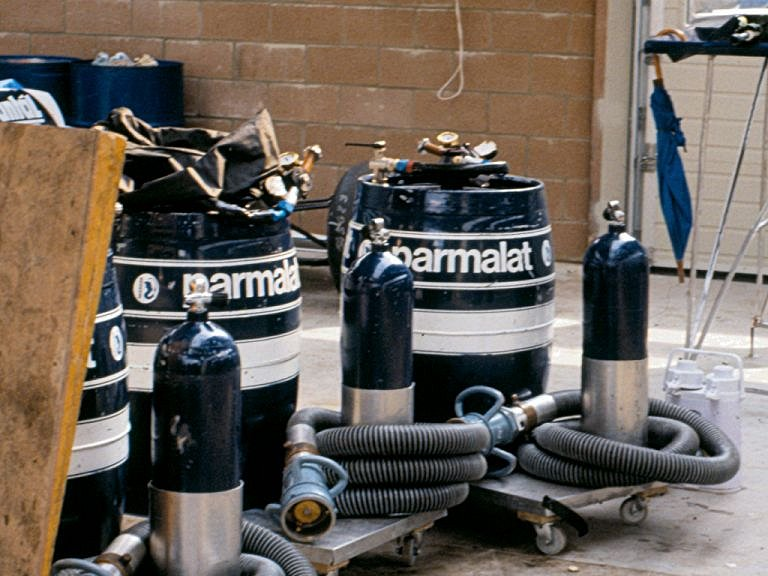
\includegraphics[width=\textwidth]{Figures/1_brabham-fuel-barrels}
\caption{Brabham's fuel tanks used to refuel during the 1982 Austrian Grand Prix. Source: \cite{Substack2024BrabhamFuelBarrelsImage}. Reproduced for educational purposes only.}
\label{image:brabham_fuel}
\end{figure}

Despite all the advances in technology, refuelling and tyres continues to be the cornerstone of race strategy. Every extra lap's worth of fuel adds weight to the car, reducing acceleration and increasing breaking distances, meaning every kilogram needs to be carefully considered. This effect is carefully calculated based on the characteristics of the car and will be a variable of race strategy optimisation models. For practical race strategy applications, this is typically approximated as linear over a stint and is considered independent from tyre degradation effects \cite{Cappello2026TyreDegradation}. Despite the current ban on mid-race refuelling applied in 2010 \cite{FIA2010SportingRegulations} these effects must be considered during non-race sessions, to find the true pace of a car independent of fuel in practice, and to achieve the lowest possible lap time without risk of running out of fuel and stopping on track to end a driver's qualifying session early. Fuel strategy represents a trade-off between lower vehicle mass and fuel saving requirements. Starting with less fuel reduces the lap time penalty associated with carrying additional mass but requires the driver to recover the fuel deficit through techniques such as lift-and-coast or reduced throttle application. Carrying additional fuel removes or reduces this requirement, allowing the driver to maintain a more aggressive driving style throughout the stint at the expense of a higher initial vehicle mass.

Tyre compound and degradation are the main strategic component of modern F1. Before the 1990s choice of tyre was more of an afterthought, with teams using mass produced road tyres which were poorly designed for racing situations - various estimates suggest ~30\% of race retirements during the 1950s and 60s were caused by tyre failures \cite{GrandPrix2472023TyreEvolution}. Various advances were made, particularly in the 1970s, with the introduction of radial tyre construction and the differentiation between slick and grooved tyres for dry and wet situations, but these did not typically provide strategic variety [x - footnote - Hunt / Lauda 1976 Japan] as each team would adopt the latest technologies. The multiple manufacturers eventually reduced during the 1990s and 2000s to various combinations of Goodyear, Bridgestone, and Michelin, which led to teams choosing dedicated tyre manufacturers which could tailor products to their needs, such as the alliance between Bridgestone and Scuderia Ferrari \cite{Bridgestone2002FerrariPartnership,Crash2005FerrariBridgestone}, and resulted in "Tyre Wars" between the manufacturers and their associated teams [x - find source] as each developed proprietary rubber compounds [x] and affected teams' abilities to compete such as the infamous 2005 Indianapolis Grand Prix where all Michelin tyre runners were required to retire due to safety concerns. The Federation Internationale de l'Automobile (FIA) eventually mandated single tyre manufacturers and introduced the modern range of dry compound tyres. 

The availability of each has varied over the years, peaking with the affectionately termed "Tyre Rainbow" of 2018 with seven distinct dry tyre compounds, before settling on picking three compounds from a pool of five (rated C1, softest, to C5, hardest) to serve as soft, medium, and hard tyres for each race in 2019 and is still the availability today. The different compounds are made of different blends of chemicals, including rubber, carbon black, silica, oils, and resins to form the chemical properties of the tyre which modify how it behaves under various lateral and longitudinal G-forces, how quickly it degrades, and how it behaves at racing temperatures.

\subsection{The Modern Pit Stop Decision}
\label{subsec:modern-pit-decision}

% HIGH PRIORITY.
% Explain the decision facing a team during a dry race:
% - continue on the current tyre;
% - stop earlier than a competitor;
% - stop later than a competitor.
% Introduce track position, tyre performance and rejoin traffic as interacting
% considerations, but do not define model parameters yet.
% End by explaining why the decision is difficult: the outcome depends on
% several time-varying and partially uncertain effects.

During a standard dry race, strategy teams need to make decisions about when the best time to commit to a pit stop is that will have the best overall impact to the driver's race time and position. A driver is required to use two distinct compounds of dry tyres under the 2026 regulations \cite{FIA2026SportingRegulations} at time of writing, meaning that at least one pit stop is required during a standard race for every driver [x - footnote - red flag rules]. This creates a set of variables that can affect the targeted lap for a pit stop.

Firstly is tyre degradation. Each tyre has an expected number of laps in its useful life as detailed in \cref{subsec:tyre-degradation-background}. If a driver stops too early in a race, the new tyre may not last until the end of the race or the next intended pit stop lap. Conversely, leaving a pit stop too late may mean the current tyre runs out of useful life causing severe time loss before the driver can return to the pits. Tyre behaviour is also a factor to consider - softer tyres typically reach their peak grip phase quicker, meaning a driver loses less time controlling a car with less grip on colder tyres. 

Competitors on the track also contribute to ideal timing for a pit stop for several reasons. Two drivers in F1 close to each other on track, on tyres of the same age and of the same tyre compound, have no differentiating factors to separate them except driver ability. However, the driver behind is driving through "dirty air", where the air coming off the car behind is washed outwards in spirals and vortexes, and does not behave smoothly providing consistent downforce as it does for the car at the front \cite{RacecarEngineering2020DirtyAir}. This makes it more difficult for the driver behind to follow closely or approach to overtake without assistance, as their car behaviour is unpredictable, leading to attempts to minimise its effect by technical regulations \cite{FIA2021ShapeThingsCome}. This is demonstrated in \cref{image:dirty_air_sim} with clean air coming in straight at the front, and appearing wavy as it comes off the back of the car. 

\begin{figure}
    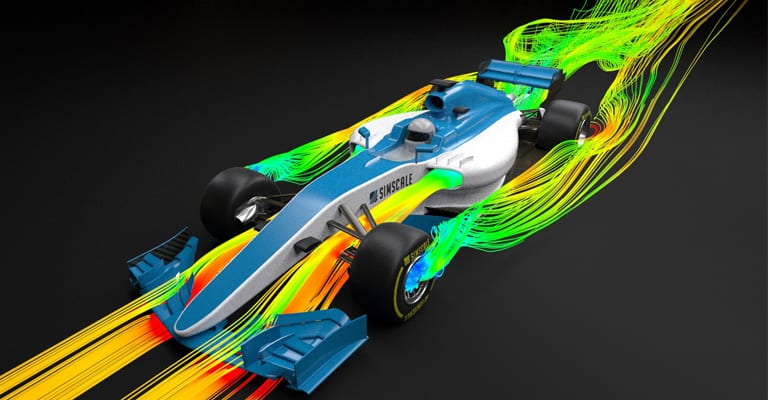
\includegraphics[width=\textwidth]{Figures/1_dirty_air_sim.jpg}
    \caption{Visualisation of the turbulent wake ("dirty air") produced behind a Formula One car. Source: \cite{SimScale2016FrontWingOptimisation}. Reproduced for educational purposes only.}
    \label{image:dirty_air_sim}
\end{figure}

By taking a pit stop, the driver behind may come out into a gap in traffic, giving them the clean air and they can go faster. They also don't lose time from defending position against drivers behind them. The reverse is also applicable; the driver behind can stay out if the driver ahead pits, freeing them into clean air and drive faster. Traffic around the pit stop procedure can impact whether this will be an effective strategy, as a driver can exit the pit lane into no gap and be unable to overtake slower moving traffic that was previously behind them.

These, amongst several other factors, are wildly fluctuating variables that impact whether a pit stop is a viable option to improve the driver's race time or to get in front of a competitor. Pure speed is not the only important outcome of a pit stop; track position can be equally important if the characteristics of a racetrack make overtaking difficult. All of these can change in a second and make a pit stop attractive or not, meaning it is incredibly difficult for the strategy engineers to attempt to predict the future and choose the best course. These variables led to the development of tactical pit stop strategies, such as the undercut.

[x - TODO - Why undercuts are difficult to analyse in retrospect, review below]

Although the outcome of an undercut is visible in historical timing data, determining why it succeeded is considerably more difficult. The observed lap time difference combines tyre degradation, compound performance, warm-up behaviour, traffic, driver pace and numerous interacting effects that cannot be directly separated. A useful engineering model must therefore estimate the contribution of each factor individually.
 
\subsection{Rise of the Undercut}
\label{subsec:rise-undercut}

% HIGH PRIORITY.
% Explain how high-degradation tyres and restricted compound allocations made
% undercuts prominent in modern F1. Cover:
% - an earlier stop exchanges temporary track position for fresher-tyre pace;
% - the gain is realised during the offset laps before the rival stops;
% - the undercut may fail through poor warm-up, traffic or insufficient delta.
% Use one or two concise historic examples if well sourced.
% Do not yet calculate the gain.

An undercut in motorsport is a strategic move which involves pitting earlier than an opponent ahead on track. This puts the driver onto fresh tyres, likely to be faster than an opponent's degraded tyres. This difference allows the driver to go faster on the out lap than the driver who was previously ahead. Even if that driver pits the following lap, this time lost means they may exit the pit lane behind the attacking driver, or so close that the driver who pit first has warmer tyres and is able to use this advantage in the corners to overtake immediately. 

The 1998 Hungarian Grand Prix is widely regarded as one of Formula One's defining strategic victories, with Ferrari using an aggressive three stop strategy to undercut the leading McLarens and secure victory despite limited overtaking opportunities \cite{Formula12020Hungary1998}. While strategic pit stop timing has influenced Formula One for decades, the removal of refuelling in 2010 placed even greater emphasis on tyre performance, making the undercut a central tactical consideration in modern race strategy.

It is important to note that this is not a guaranteed method of overtaking. Poor tyre warm-up on the outlap, the impact of traffic (both for the attacking and target driver), or attempting the undercut from too far back (so unable to close the gap even in perfect conditions) can all cause the attempt to fail and the situation on track remains unchanged. The driver ahead may also choose to stay out and build up tyre delta. When they eventually do pit, they'll have tyres several laps newer than the driver who attempted the undercut. Even if they are behind, their newer tyres will give an advantage attempting to overtake, meaning the advantage of the undercut is countered.

\section{Tyre Behaviour Relevant to Strategy}
\label{sec:tyre-behaviour-background}

% This is a focused literature-backed section, not a tyre-engineering textbook.
% Explain only the tyre behaviour needed to justify the later model.

\subsection{Tyre Compounds and Performance Trade-Off}
\label{subsec:tyre-compounds}

% HIGH PRIORITY.
% Explain the relative pace/durability trade-off between nominated compounds,
% without assuming that the soft is always strategically preferable.
% Mention that the actual performance delta is event- and condition-dependent.
%
% SUGGESTED FIGURE 1.1:
% Conceptual compound pace versus durability diagram.
% Mark as conceptual rather than measured data.

 \cref{fig:1_conceptual_tyres} shows how different tyre compounds affect tyre life and behaviour at an abstract level. A softer tyre typically has more grip, being able to warm up to racing temperatures more quickly and mould to the granularity of the road, but degrades more quickly as the rubber is pulled apart by the tarmac, making it the preferred tyre for single-lap pace in qualifying. The harder tyre is the reverse, being longer and more durable while sacrificing higher grip, making it more suitable for longer race stints \cite{RaceTeq2024TyreDegradation,Taylor2020FrictionRacingTyres,RacecarEngineering2020TyreGrip}.

\begin{figure}[htbp]
\centering
\begin{tikzpicture}
\begin{axis}[
    width=0.85\textwidth,
    height=0.5\textwidth,
    xlabel={Tyre Age (laps)},
    ylabel={Conceptual Lap Time (s)},
    xmin=1,
    xmax=45,
    ymin=60,
    ymax=120,
    ytick={60,70,80,90,100,110,120},
    xtick={1,5,10,15,20,25,30,35,40,45},
    ymajorgrids=true,
    grid style=dashed,
    legend style={
        at={(0.5,1.02)},
        anchor=south,
        legend columns=3,
        draw=none
    },
    tick align=outside
]

% Soft
\addplot[
    thick,
    red,
    smooth,
    mark=*,
    mark size=1.8pt
] coordinates {
(1,65)
(3,61)
(5,61)
(10,65)
(14,69)
(16,73)
(17,77)
(18,82)
(19,87)
(20,92)
(21,97)
(22,102)
(23,107)
(24,112)
(25,117)
};
\addlegendentry{Soft}

% Medium
\addplot[
    thick,
    yellow!70!black,
    smooth,
    mark=*,
    mark size=1.8pt
]  coordinates {
(1,70)
(3,66)
(7,66)
(12,69)
(17,72)
(22,75)
(27,78)
(28,82)
(29,88)
(30,93)
(31,98)
(32,102)
(33,107)
(34,112)
(35,117)
};
\addlegendentry{Medium}

% Hard
\addplot[
    thick,
    black!65,
    smooth,
    mark=*,
    mark size=1.8pt
]  coordinates {
(1,75)
(3,71)
(9,71)
(14,72)
(19,73)
(24,74)
(29,75)
(34,76)
(38,77)
(40,82)
(41,87)
(42,92)
(43,97)
(44,102)
(45,107)
(46,112)
(47,117)
};
\addlegendentry{Hard}

\end{axis}
\end{tikzpicture}
\caption{Conceptual tyre degradation curves used by the strategy model. Soft tyres provide the greatest initial performance but degrade most rapidly, while hard tyres exhibit the lowest initial performance and slowest degradation.}
\label{fig:1_conceptual_tyres}
\end{figure}

 The actual delta in grip and life varies depending on the circuit and event. Circuit racetrack surfaces vary in composition, finish quality, and granularity of the stones that make it up. All of these properties combine to create a particular roughness to the track surface, which in turn affects how a tyre moulds to grip it and how the tyre degrades each lap \cite{RacecarEngineering2020TyreGrip}. Additionally, ambient conditions, particularly track surface temperature, influence tyre behaviour. Increasing track temperature generally increases grip by bringing the tyre closer to its optimum operating window; however, excessive temperatures can lead to overheating, causing grip to decline and degradation to accelerate \cite{RacecarEngineering2008EssenceGrip}. 

\subsection{Tyre Degradation}
\label{subsec:tyre-degradation-background}

% VERY HIGH PRIORITY -- this literature directly supports Chapter 3.
% Distinguish where useful:
% - wear/mechanical degradation;
% - thermal degradation;
% - progressive pace loss;
% - severe non-linear loss or a tyre 'cliff'.
% Explain why degradation creates a fresh-versus-old tyre performance delta.
% Discuss whether short sections of a stint may reasonably be approximated as
% linear, while acknowledging that real behaviour is not universally linear.
% Save the chosen mathematical formulation for Chapter \ref{chap:model}.

As the car progresses through the race, the tyre will degrade as bits of rubber called marbles are torn off from the surface of the tyre and deposited onto the racetrack as seen in \cref{image:track_marbles}. These will collect and build up over the course of the race. As the tyre falls apart in this way, it causes reduced cornering speeds, reduced traction, and increased braking distances, all adding to a reduction in lap time. This can make overtaking later in the race riskier and more difficult, as the marbles can attach back to a tyre driving over them as seen in \cref{image:tyre_marbles}. This causes an uneven surface to the tyre, meaning grip is less optimised and the car may behave unpredictable when braking or lacking grip as it traverses the corner. This can make pit stop strategies more appealing as it reduces the risk of factors on the race track affecting the outcome of the manoeuvre. 

\begin{figure}
    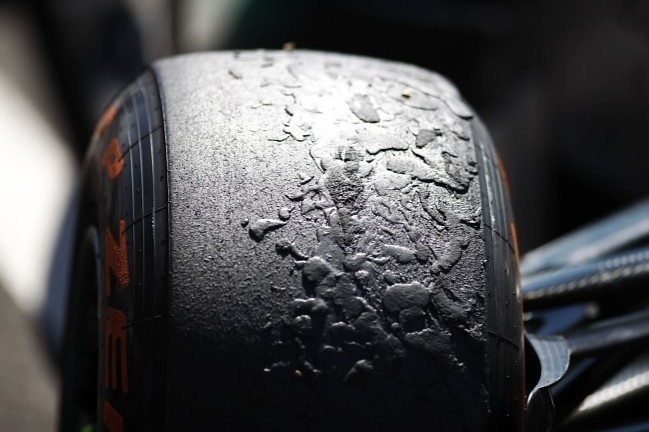
\includegraphics[width=\textwidth]{Figures/1_tyre_marbles.jpg}
    \caption{When a racer drivers over tyre marbles, the heat can cause them to attach to the tyre, causing it to be uneven and negatively impacting grip. Source: \cite{F1Technical2013TyreMarbles}. Reproduced for educational purposes only.}
    \label{image:tyre_marbles}
\end{figure}

\begin{figure}
    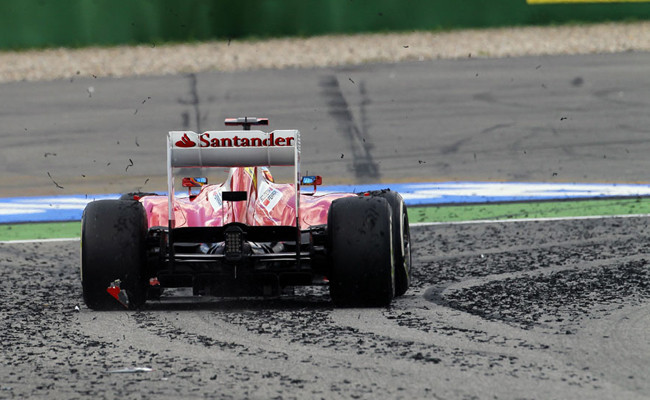
\includegraphics[width=\textwidth]{Figures/1_marbles_on_track.jpg}
    \caption{As the tyre degrades, chunks of rubber called marbles break off and start to collect off the racing line, typically on the outside of corners. Source: \cite{MotorPasion2014Marbles}. Reproduced for educational purposes only.}
    \label{image:track_marbles}
\end{figure}

The tyre is affected by mechanical and thermal degradation. Mechanical degradation refers to the physical characteristics of the tyre and how these wear due to repeated contact with the track. The tyre suffers significant shear forces (parallel to the surface) which cause parts of the material to slide against and alongside each other and remove rubber from the contact patch. This reduces the tyre's ability to conform the the microscopic grain of the racetrack surface and lowers the available grip \cite{Taylor2020FrictionRacingTyres}. The rate at which this occurs is influenced by several factors such as tyre compound, vehicle setup, driver inputs, track temperature, or circuit abrasiveness \cite{RacecarEngineering2020TyreGrip}. How each of these factors individually contributes is beyond the scope of this research, but the important consequence from a strategic perspective is that tyre grip degrades gradually throughout a race stint bringing a gradual reduction in lap time. Mechanical wear is generally progressive rather than instantaneous, meaning that over relatively short sections of a stint the associated loss of performance may be approximated using simplified degradation models. This assumption is explored further in Chapter 3 when selecting an appropriate representation for lap time prediction.

In parallel to this, thermal degradation describes the reduction in tyre performance caused by operating outside of its optimal operating window. The tyre builds temperature on the surface and inside the carcass as the tyre undergoes repeated cycles of braking, acceleration, and cornering. If the tyre exceeds its intended operational temperatures, the rubber compound in the tyre breaks down and loses its mechanical properties, causing reduced grip even if there is plenty of tyre rubber still available. Unlike purely mechanical wear, thermal degradation can therefore produce a noticeable reduction in performance without substantial physical loss of rubber.

In practice, tyre performance is rarely governed by a single degradation mechanism. Mechanical wear and thermal degradation occur simultaneously, with their relative importance varying according to the tyre compound, circuit characteristics, environmental conditions and driver behaviour. Rather than attempting to model these mechanisms independently, race strategy tools typically represent their combined effect through changes in lap time performance, as this is the quantity directly relevant to strategic decision making.

A racecar tyre typically shows four informally designated distinct phases of degradation over its lifetime \cite{Cappello2026TyreDegradation}, shown in \cref{fig:1_tyre_life} as a conceptual graph comparing age of the tyre in laps to a theoretical lap time in seconds. Each affects how the tyre behaves on the racetrack:
\begin{itemize}
    \item Ramping up: The tyre takes a small number of laps to reach its ideal operating temperature (lap 1-3). This process can be shortened by initially fitting the tyre at a higher temperature; F1 achieves this with tyre warming blanket which heat dry \& intermediate tyres to 70 degrees Celcius ({\degree}C) and wet tyres to 40 {\degree}C before being attached to the car.
    \item Peak Grip: The tyre is in its peak operating window (lap 3-15). Lap time degradation is slow and the tyre offers the best lap time. 
    \item Degradation: The tyre is no longer optimal, but is still providing competitive lap times (lap 15-45). The tyre will typically lose small amounts of lap time each lap, rather than hover around a consistent time. 
    \item The Cliff: The structural integrity of the tyre has failed and is essentially unusable for any competitive laps (lap 45 onwards). Lap times get much slower lap on lap and a puncture is not only risky but likely.
\end{itemize}

\begin{figure}[htbp]
\centering
\begin{tikzpicture}
\begin{axis}[
    width=0.85\textwidth,
    height=0.5\textwidth,
    xlabel={Tyre Age (laps)},
    ylabel={Conceptual Lap Time (s)},
    xmin=1,
    xmax=50,
    ymin=60,
    ymax=120,
    ytick={60,70,80,90,100,110,120},
    xtick={1,3,5,10,15,20,25,30,35,40,45,50},
    ymajorgrids=true,
    grid style=dashed,
    legend style={
        at={(0.5,1.02)},
        anchor=south,
        legend columns=3,
        draw=none
    },
    tick align=outside
]

% Soft
\addplot[
    thick,
    red,
    mark=*,
    mark size=1.8pt
] coordinates {
(1,70)
(3,61)
(5,61.15)
(10,61.6)
(15,62)
(20,65)
(25,68)
(30,71)
(35,74)
(40,77)
(45,80)
(46,85)
(47,90)
(48,95)
(49,100)
(50,105)
};

\end{axis}
\end{tikzpicture}
\caption{Conceptual tyre degradation model of tyre lifecycle, demonstrating the four distinct phases of tyre behaviour - ramping up (laps 1-3), peak grip (laps 3-15), degradation (laps 15-45), and the cliff (laps 45-50).}
\label{fig:1_tyre_life}
\end{figure}

The impact of tyre degradation has a strong impact on choosing optimum pit stop times. A tyre that is rapidly degrading or approaching the final stage of its life significantly reduces the range of options for bringing the driver in for a tyre change. They need to be able to make the new tyre last until the end of the race or the intended stint. Pitting too many times will result in an unacceptable loss of race time even if the new tyres are theoretically much quicker. Strategists need to balance the physical tyre characteristics with the driver's abilities to control the behaviour of the tyre during its life to determine the ideal strategic option.

\subsection{Tyre Warm-Up and Out-Lap Performance}
\label{subsec:tyre-warmup-background}

% HIGH PRIORITY if warm-up is included in the model; MEDIUM otherwise.
% Explain why a newly fitted tyre may not deliver peak pace immediately.
% Relate this to undercut failure and overcut opportunity.
% Avoid implementation details and numerical assumptions here.

The out-lap is the first lap on a new tyre when leaving - or coming out of - the pit lane. This is one of the most critical periods of an undercut manoeuvre as the driver pitting driver needs to optimise their lap time so that, when the competitor does pit, they will come out behind. As discussed in \cref{subsec:tyre-degradation-background} the initial phase includes tyre warm-up to reach peak performance. This can result in failure to cut, resulting in an overcut for the defending driver where they manage to go longer with their stint and stay ahead.

In addition to the physical characteristics of the tyre, and how these change throughout a stint, the behaviour of the tyre can be controlled by the driver with their driving style or changes to the balance of the car. For example, a driver in a modern F1 car is able to adjust the balance of braking force longitudinally the car, meaning different amounts of braking forces are applied to front and rear tyres. The driver can also bring the tyre temperature to optimum faster with particular driving techniques, such as more pressure on the brakes to reduce the required braking distance. The sooner the tyre reaches peak performance, the best lap time the driver will have available for the crucial out-lap.

\section{Pit Stop Strategy Scenarios}
\label{sec:pit-stop-scenarios}

% PURPOSE: provide a common vocabulary for readers who may understand
% motorsport engineering but not race-strategy terminology.
% Keep each scenario concise and observational: what happens on track, what the
% team is trying to achieve, and which broad conditions favour it.

\subsection{Stay Out}
\label{subsec:stay-out}

% Explain:
% - the driver retains track position and continues on the current tyre;
% - potential reasons: clean air, avoiding traffic, extending to a preferred
%   compound/window, low degradation, or preserving strategic flexibility;
% - risks: worsening pace, exposure to an undercut, or reaching the tyre cliff.

\subsection{Undercut}
\label{subsec:undercut-background}

% Explain:
% - the attacking driver stops first;
% - the target remains on older tyres;
% - the attacker attempts to gain sufficient time before the target stops;
% - success is judged after the target's corresponding stop/rejoin.
% Mention broad favourable conditions: meaningful fresh-tyre delta, rapid
% warm-up, clear rejoin and sufficient offset time.
%
% SUGGESTED FIGURE 1.2 -- HIGH VALUE:
% A simple two-driver timeline showing pit order, offset laps and rejoin.

\subsection{Overcut}
\label{subsec:overcut-background}

% Explain:
% - the attacking/leading driver remains out after the rival stops;
% - it can work when old tyres remain competitive or the rival has a poor
%   out-lap, warm-up difficulty or traffic;
% - it is strategically relevant even if not a primary implemented output.
% Clarify later scope in Chapter \ref{chap:problem}.

\section{Existing Research and Modelling Approaches}
\label{sec:existing-research}

% VERY HIGH PRIORITY ACADEMIC SECTION.
% This is the integrated literature review thread. Direct papers specifically
% about F1 undercuts may be sparse; review the components instead:
% - race-strategy simulation and optimisation;
% - lap time and stint time modelling;
% - tyre degradation estimation from telemetry/timing data;
% - deterministic versus probabilistic strategy methods;
% - use of historical race data for validation.
%
% For each source, do more than summarise:
% - identify the method;
% - identify the useful contribution;
% - identify limitations for this project;
% - state how it informs the chosen approach.
%
% SUGGESTED TABLE 1.1:
% Source | Problem | Method | Relevant finding | Limitation / use here.
% This can efficiently demonstrate comparison rather than a source-by-source
% narrative.

[x - TODO - REVIEW AI WRITTEN TEXT]

Existing Formula One race strategy research has predominantly approached pit stop timing as a complete race optimisation problem. Proposed solutions range from discrete-event simulation and dynamic programming to
Monte Carlo planning, game theory and machine learning. Although these approaches differ in their treatment of uncertainty, competition and decision making, they share a common objective of determining an optimal
race strategy over an entire Grand Prix rather than evaluating an individual strategic opportunity.

Table \ref{tab:existing_research} summarises the principal approaches identified in the literature and their relevance to the present work.

\begin{table}[htbp]
\centering
\caption{Comparison of Formula One race strategy modelling approaches.}
\label{tab:existing_research}

\small
\renewcommand{\arraystretch}{1.25}

\begin{tabularx}{\textwidth}{|
>{\raggedright\arraybackslash}p{0.21\textwidth}|
>{\raggedright\arraybackslash}p{0.18\textwidth}|
>{\raggedright\arraybackslash}p{0.16\textwidth}|
X|
}
\hline
\textbf{Source}
&
\textbf{Method}
&
\textbf{Scope}
&
\textbf{Relevance to this project}
\\
\hline

Bekker \& Lotz
\cite{BekkerLotz2009}
&
Discrete-event simulation
&
Whole-race strategy
&
Demonstrates historical race simulation and validation against real race outcomes, supporting the use of simulation as a decision-support tool.
\\
\hline

Carrasco Heine \& Thraves
\cite{CarrascoHeineThraves2023}
&
Dynamic programming
&
Whole-race optimisation
&
Models tyre wear and cumulative race time. Supports lap time based optimisation but not isolated undercut analysis.
\\
\hline

Piccinotti
\cite{Piccinotti2021}
&
Monte Carlo planning
&
Whole-race planning
&
Uses historical race data and probabilistic simulation to evaluate strategic options under uncertainty.
\\
\hline

Aguad \& Thraves
\cite{AguadThraves2024}
&
Dynamic programming and game theory
&
Two-driver interaction
&
Introduces direct interaction between competing drivers, conceptually similar to the two-driver comparison considered in this work.
\\
\hline

Thomas et al.
\cite{ThomasEtAl2025}
&
Explainable reinforcement learning
&
Whole-race optimisation
&
Demonstrates modern AI-based strategy optimisation while maintaining model interpretability.
\\
\hline

Hettmann
\cite{Hettmann2024}
&
Machine learning
&
Pit stop prediction
&
Predicts pit stop timing from historical races rather than evaluating the engineering causes of successful undercuts.
\\
\hline

Fatima \& Johrendt
\cite{FatimaJohrendt2023}
&
Deep neural networks
&
Race outcome prediction
&
Illustrates the increasing application of deep learning to Formula One strategy, although with limited transparency.
\\
\hline

\end{tabularx}

\end{table}

The earliest work identified is that of Bekker and Lotz \cite{BekkerLotz2009}, who demonstrated that Formula One race strategy could be represented using discrete-event simulation. Their model incorporated pit stops, overtaking and race interruptions before validating the resulting simulator against three historic Grands Prix. Although based on regulations that pre-date the modern tyre-focused era, the work established simulation as a viable methodology for evaluating race strategy using historical data.

Subsequent research has generally shifted towards optimisation rather than simulation alone. Carrasco Heine and Thraves \cite{CarrascoHeineThraves2023} formulate race strategy as a dynamic programming problem, minimising cumulative race time while accounting for tyre degradation, compound selection and stochastic events such as yellow flags. Aguad and Thraves \cite{AguadThraves2024} extend this concept by modelling strategic interaction between competing drivers using a Stackelberg feedback game. These approaches demonstrate that race strategy can be formulated as a mathematical optimisation problem but are primarily concerned with determining globally optimal race strategies rather than evaluating an individual undercut opportunity.

More recent work has increasingly adopted machine learning techniques. Hettmann \cite{Hettmann2024} predicts pit stop timing using supervised learning and driver clustering, while Fatima and Johrendt \cite{FatimaJohrendt2023} employ deep neural networks to predict race outcomes and strategic decisions. Thomas et al. \cite{ThomasEtAl2025} further demonstrate that reinforcement learning can produce competitive race strategies while retaining a degree of interpretability through explainable artificial intelligence techniques. These approaches illustrate the predictive capability of data-driven models but generally sacrifice the transparency offered by deterministic engineering models.

A complementary direction is represented by Piccinotti \cite{Piccinotti2021}, who combines historical Formula One data with Monte Carlo simulation to explore race strategies under uncertainty. By sampling many possible race evolutions, the model accounts for uncertainty in competitor behaviour and race events. This probabilistic approach contrasts with the present work, which deliberately considers a deterministic retrospective scenario in which the observed race provides the complete set of external conditions.

Collectively, these studies demonstrate that Formula One race strategy has been successfully modelled using a wide range of optimisation, simulation and machine learning techniques. However, the overwhelming majority seek to optimise or predict complete race strategies. Relatively little attention has been given to the isolated engineering problem of evaluating whether a specific undercut opportunity existed at a particular point during a race.

Consequently, this dissertation adopts a deliberately narrower scope. It does not attempt to determine the globally optimal race strategy or predict competitor behaviour. Instead, it develops a transparent, deterministic model that compares two observed drivers over a local decision window, allowing the contribution of tyre degradation, compound performance, warm-up effects and traffic to be examined individually. This positions the work between descriptive historical analysis and complete race-strategy optimisation while maintaining direct interpretability of every modelling assumption.

[x - TODO - REVIEW AI WRITTEN TEXT]

\section{Research Gap and Project Motivation}
\label{sec:research-gap}

% VERY HIGH PRIORITY -- final section of Chapter 1.
% Synthesise the literature and context into a clear gap. Avoid claiming that
% no undercut tools exist unless this can be evidenced.
%
% A defensible framing might be:
% - professional teams use sophisticated proprietary strategy systems;
% - public research often treats whole-race optimisation or individual tyre
%   effects rather than an explainable undercut-focused comparison;
% - there is value in a transparent, configurable and historically validated
%   model showing how individual assumptions affect predicted undercut gain.
%
% End with a transition to Chapter \ref{chap:problem}, which formalises the aim,
% objectives, scope and success criteria.

The preceding sections demonstrate that Formula One race strategy has received considerable academic attention. Existing work has successfully applied discrete-event simulation, dynamic programming, game theory, Monte Carlo methods and machine learning to optimise race strategy, predict pit stop timing and improve race outcomes. These studies demonstrate that race strategy is a suitable domain for mathematical modelling and provide a strong methodological foundation for future research.

Despite this breadth of research, the majority of published work treats pit stop timing as part of a complete race optimisation problem. Simulation models generally seek to determine an optimal race strategy, while machine learning approaches attempt to predict competitor actions or race outcomes. Consequently, comparatively little attention has been given to analysing individual strategic opportunities within an observed race using a transparent and explainable engineering model.

The undercut represents one of the most influential tactical decisions available during a Formula One race. While its effectiveness is widely recognised within professional motorsport, evaluating whether an undercut opportunity genuinely existed requires consideration of tyre degradation, compound performance, warm-up behaviour, traffic and other interacting factors. Existing optimisation frameworks naturally include many of these effects, but they do not typically isolate the undercut as an engineering problem in its own right or provide clear visibility of how individual assumptions influence the predicted outcome.

This dissertation therefore adopts a deliberately narrower scope than much of the existing literature. Rather than predicting complete race strategies or replacing the judgement of race engineers, it develops a deterministic model that evaluates historical undercut opportunities between two observed drivers. By exposing the principal modelling parameters and validating the resulting predictions against historical race data, the model provides a transparent framework through which the effect of individual engineering  assumptions can be examined and understood.

The remainder of this dissertation formalises this objective. Chapter \ref{chap:problem} defines the research aims, objectives, project scope and success criteria before introducing the assumptions that underpin the proposed modelling approach.
\chapter{Problem Definition}
\label{chap:problem}

% ============================================================================
% CHAPTER PURPOSE -- HIGH PRIORITY
% Convert the research context into a precise, assessable project. This chapter
% must define the problem, aim, objectives, deliverables, boundaries and success
% criteria before the model is introduced.
% Do not repeat the background and do not introduce detailed equations.
% ============================================================================

\section{Problem Statement}
\label{sec:problem-statement}

% VERY HIGH PRIORITY.
% State the engineering problem in operational terms. For example:
% During a race, a team must determine whether stopping before a nearby rival
% will generate enough time during the offset laps to change the post stop
% running order, while accounting for tyre state and other relevant effects.
%
% Clarify that the problem is not merely to predict a lap time. It is to compare
% two counterfactual strategy scenarios over a defined time horizon.
% Explain the need for transparency: the user should be able to identify which
% factors produced the recommendation.

\section{Research Aim}
\label{sec:research-aim}

% State one concise aim, ideally a single sentence. Suggested form:
% "To develop, implement and validate a deterministic model for quantifying the
% time gain or loss associated with Formula One undercut opportunities using
% historic lap time data and configurable race parameters."
% Adapt only once the exact final scope is fixed.

[x - Come back at end, check this matches the final product]

This research aims to develop, implement, and validate a deterministic model for quantifying the time gain or time loss associated with Formula One undercut opportunities in race strategies. This will use configurable race and track parameters to identify opportunities, and validate against dynamically retrieved historic lap time data.

\section{Research Objectives}
\label{sec:research-objectives}

% VERY HIGH PRIORITY. Use an enumerated list so Chapter 7 can revisit each item.
% Each objective must be specific enough to assess.
%
% Suggested objectives:
% \begin{enumerate}
%   \item Identify and justify the principal factors influencing undercut gain.
%   \item Develop a progressive lap time and scenario-comparison model.
%   \item Implement the model in a desktop engineering-analysis tool.
%   \item Visualise predicted opportunities on historic race traces.
%   \item Verify the mathematical and software implementation.
%   \item Validate the model against selected historic F1 undercut cases.
%   \item quantify sensitivity to the principal model parameters and critically
%         evaluate applicability and limitations.
% \end{enumerate}
%
% Avoid objectives such as "research tyres" that are activities rather than
% assessable outcomes.

\begin{enumerate}
    \item Identify and justify the factors influencing time gain and loss of an undercut manoeuvre, including the level at which each can impact.
    \item Develop a progressive lap time model than encompasses these factors and can be used to compare various scenarios.
    \item Implement the model in a desktop software tool for engineer analysis.
    \item Visualise the analysis and predicted opportunities on historic race traces.
    \item Verify the mathematical and software implementation.
    \item Identify and select a representative range of successful and unsuccessful historic F1 undercut scenarios.
    \item Validate the model against selected historic F1 undercut cases.
    \item Critically evaluate the applicability, sensivity, and limitations of the final model and software solution.
\end{enumerate}

\section{Research Questions}
\label{sec:research-questions}

% HIGH VALUE. A short set of questions sharpens the dissertation argument.
% Suggested questions:
% RQ1: Can a deterministic model reproduce the direction and approximate
%      magnitude of undercut gain observed in historic races?
% RQ2: Which parameters exert the greatest influence on predicted gain?
% RQ3: Under which conditions does the simplified model become unreliable?
% Align results subsections directly to these questions.

\begin{enumerate}[label=\textbf{RQ\arabic*:}]
    \item Can a deterministic model reproduce the direction and approximate magnitude of undercut gain observed in historic Formula One races?
    \item Which model parameters exert the greatest influence on predicted undercut gain or loss?
    \item Under which racing conditions does the proposed modelling approach become unreliable?
\end{enumerate}

\section{Project Deliverables}
\label{sec:deliverables}

% Distinguish research/engineering artefacts from software artefacts.
%
% Research and engineering deliverables:
% - documented model formulation;
% - parameter definitions and assumptions;
% - verification and validation method;
% - sensitivity and limitations analysis.
%
% Software deliverables:
% - desktop application containing the model;
% - historic session/driver loading;
% - configurable parameters;
% - race trace output with pit/opportunity annotations.
%
% Do not let the software list dominate the engineering deliverables.

Collectively, these deliverables provide both the engineering artefacts
required to evaluate the proposed modelling approach and a practical
software implementation capable of applying the model to historic Formula
One race data.

\subsection{Research \& Engineering Deliverables}
\label{subsec:research-deliberables}

\begin{itemize}
    \item A documented deterministic undercut model.
    \item A definition and justification of all model parameters and assumptions.
    \item A documented verification and validation methodology.
    \item Validation results using historic Formula One races.
    \item A sensitivity analysis and critical discussion of model limitations.
\end{itemize}

\subsection{Software Deliverables}
\label{subsec:software-deliverables}

\begin{itemize}
    \item A desktop engineering analysis application implementing the proposed model.
    \item Historic race loading and session selection functionality.
    \item Configurable engineering parameters.
    \item Race trace visualisation with annotated pit stops and predicted undercut opportunities.
\end{itemize}

\section{Project Scope and Boundaries}
\label{sec:scope}

\subsection{Included Scope}
% Define the intended operating domain precisely. Candidate boundaries:
% - Formula One race sessions using historic timing/lap data;
% - dry, green-flag running unless otherwise explicitly analysed;
% - one attacking driver and one target driver;
% - short offset windows around a pit stop decision;
% - deterministic output based on supplied/estimated parameters;
% - undercut as the principal strategy mechanism.

\begin{itemize}
    \item Historic Formula One race sessions using publicly available timing and lap data.
    \item Dry race conditions under uninterrupted green-flag running.
    \item Comparison between a single attacking driver and a single target driver.
    \item Analysis of local decision windows surrounding an undercut opportunity.
    \item Deterministic prediction using configurable engineering parameters.
    \item Evaluation of the undercut as the primary strategic manoeuvre.
\end{itemize}

\subsection{Excluded Scope}
% Explicitly list exclusions and give one sentence of rationale where needed:
% - complete whole-race strategy optimisation;
% - Safety Car, VSC, red flag and weather transitions;
% - mechanical failures, team orders and driver intent;
% - stochastic prediction of future incidents;
% - proprietary team telemetry or confidential strategy methods;
% - live operational use, unless actually implemented and validated.
% Overcut may be contextual/future work rather than a full primary output.

\begin{itemize}
    \item Complete race strategy optimisation.
    \item Safety Car, Virtual Safety Car and red-flag periods.
    \item Wet-weather transitions and changing track conditions.
    \item Mechanical failures and reliability-related retirements.
    \item Team orders and strategic intent.
    \item Prediction of future race incidents.
    \item Proprietary telemetry and confidential Formula One team strategy systems.
    \item Live race support or operational deployment.
\end{itemize}

\section{Success Criteria}
\label{sec:success-criteria}

% VERY HIGH VALUE and currently missing from the earlier scaffold.
% Define how success will be judged before results are known.
% Use measurable or at least auditable criteria, for example:
% - equations and scenario logic pass defined verification tests;
% - model produces physically/strategically sensible monotonic behaviour;
% - predicted sign of gain/loss agrees with selected historic cases;
% - prediction error is reported using a defined metric;
% - parameter sensitivity is quantified rather than described informally;
% - the race trace enables prediction and actual outcome to be compared.
% Do not invent an arbitrary accuracy threshold unless justified.

\begin{enumerate}
    \item The mathematical formulation shall be successfully verified.
    \item The software implementation shall correctly reproduce the mathematical model.
    \item The model shall produce physically plausible behaviour when principal parameters are varied.
    \item The model shall reproduce the direction of gain or loss observed in selected historic undercut scenarios.
    \item Prediction error shall be quantified using appropriate performance metrics.
    \item Model sensitivity shall be analysed for the principal configurable parameters.
    \item The software shall provide a race trace visualisation capable of comparing predicted and observed outcomes.
\end{enumerate}

\section{Assumptions}
\label{sec:project-assumptions}

% Provide only project-level assumptions here; Chapter \ref{chap:model} gives
% the mathematical consequences of each assumption.
% Candidate assumptions:
% - historic timing data are sufficiently accurate for the intended analysis;
% - representative base pace and degradation estimates can be obtained;
% - equivalent pit-lane loss for both drivers in the symmetric comparison;
% - no disruptive race-control event during the comparison window;
% - driver/car performance can be represented by an explicit pace offset where
%   required;
% - the decision is based on cumulative time, not on guaranteed overtaking.

\begin{itemize}
    \item Historic timing data are sufficiently accurate for retrospective analysis.
    \item Representative degradation rates can be estimated for each tyre compound.
    \item Pit-lane transit time is assumed equal for both drivers unless otherwise stated.
    \item No Safety Car, Virtual Safety Car or red-flag period occurs during the comparison window.
    \item Relative driver pace can be represented by configurable pace offsets.
    \item The outcome of an undercut is evaluated using cumulative race time rather than the probability of completing an overtake on track.
\end{itemize}

\section{Project Plan and Milestones}
\label{sec:project-plan}

% HIGH PRIORITY if required by the project/report brief; otherwise concise.
% Update dates to reflect the leave of absence and actual revised schedule.
% Include:
% - model definition freeze;
% - minimum model implementation;
% - data ingestion/race trace;
% - verification;
% - historic validation;
% - sensitivity analysis;
% - report completion and contingency.
%
% SUGGESTED FIGURE 2.1 / APPENDIX:
% Revised Gantt chart. Keep detailed task notes in an appendix if too large.
% Explain deviations from the original plan later in Chapter 4 or evaluation,
% rather than pretending the original dates remained valid.

\section{Risk Management}
\label{sec:risk-management}

% HIGH VALUE and was absent from the earlier scaffold.
% Add a concise risk table:
% Risk | Likelihood | Impact | Mitigation | Residual risk.
% Include at minimum:
% - insufficient/poor-quality historic data;
% - API changes or rate limits;
% - model complexity exceeding available time;
% - inability to validate a parameter directly;
% - overfitting conclusions to a small number of race cases;
% - software failure or source loss;
% - personal/time constraints following the revised project schedule.
% Keep personal detail professional and proportionate.

\begin{table}[htbp]
\centering
\caption{Project risk assessment and mitigation measures.}
\label{tab:project-risks}

\small
\renewcommand{\arraystretch}{1.3}

\begin{tabularx}{\textwidth}{|
>{\raggedright\arraybackslash}p{0.25\textwidth}|
>{\centering\arraybackslash}p{0.10\textwidth}|
>{\centering\arraybackslash}p{0.10\textwidth}|
X|
>{\centering\arraybackslash}p{0.12\textwidth}|}
\hline

\textbf{Risk} &
\textbf{Likelihood} &
\textbf{Impact} &
\textbf{Mitigation} &
\textbf{Residual Risk}
\\
\hline

Insufficient or poor-quality historic race data &
Medium &
High &
Use multiple publicly available data sources (FastF1, OpenF1 and FIA timing where appropriate), validate imported data, and select alternative race case studies if necessary. &
Low
\\
\hline

API changes, outages or rate limits preventing data retrieval &
Medium &
Medium &
Cache downloaded sessions locally, abstract API access within the software, and support loading previously downloaded data. &
Low
\\
\hline

Model complexity exceeds the available project timescale &
Medium &
High &
Develop the model progressively, beginning with a simple deterministic formulation before incrementally introducing additional factors. Prioritise validation over unnecessary complexity. &
Low
\\
\hline

Unable to directly validate individual model parameters &
High &
Medium &
Justify parameter values using published literature, engineering judgement and sensitivity analysis rather than relying solely on direct measurement. &
Medium
\\
\hline

Conclusions influenced by too few historic race case studies &
Medium &
High &
Validate against multiple races, circuits and tyre strategies where practical, and explicitly discuss limitations on the generalisability of the results. &
Medium
\\
\hline

Loss or corruption of software source code &
Low &
High &
Maintain version-controlled source code with regular remote backups and incremental commits throughout development. &
Low
\\
\hline

Project progress affected by time constraints &
Medium &
High &
Prioritise completion of the core deterministic model and validation before implementing optional functionality. Defer lower-priority enhancements to future work where necessary. &
Low
\\
\hline

\end{tabularx}
\end{table}

\section{Chapter Summary}
\label{sec:problem-summary}

% One short paragraph only:
% - restate what has been bounded;
% - identify the resulting modelling task;
% - transition to Chapter \ref{chap:model}.

\chapter{Model Development}
\label{chap:model}

% ============================================================================
% CHAPTER PURPOSE -- VERY HIGH PRIORITY / TECHNICAL CORE
% Construct the undercut analysis methodology from the engineering question to
% the final cumulative scenario comparison. The reader should understand what
% is compared, over which interval, and why each model term is required before
% encountering the fully indexed formulation.
%
% Narrative order:
% race state -> terminology -> scenarios -> comparison window -> lap time
% prediction -> model extensions -> cumulative comparison -> decision metrics.
% ============================================================================

\section{Modelling Approach}
\label{sec:modelling-approach}

% Keep this opening conceptual. Detailed equations begin only after the reader
% understands the two hypothetical futures and their common time window.

The model evaluates whether an attacking driver would gain or lose time by
making a pit stop at a selected point in a historic race. It is deterministic:
the same reference race state and parameter values always produce the same
result. It is also comparative rather than predictive of the complete race.
Two hypothetical futures are generated from one decision point and evaluated
over a common time interval:

\begin{itemize}
    \item In the \emph{stay out scenario}, the attacking driver remains on the
    current tyre at the decision point.
    \item In the \emph{undercut scenario}, the attacking driver pits at the
    decision point and continues on the specified replacement tyre.
\end{itemize}

The target driver's assumed behaviour is common to both scenarios. This
isolates the effect of the attacking driver's decision rather than attributing
the result to an abnormal stop or an unrelated change in the target driver's
pace. Lap times are predicted individually and accumulated over a defined
comparison window. The principal output is a continuous time gain or loss; the
corresponding track-position outcome is reported separately.

The method is intended to capture the dominant tyre-driven mechanism of an
undercut while remaining explainable and suitable for sensitivity analysis. It
does not attempt to reproduce the stochastic behaviour of a complete Formula
One race or replace the broader judgement required by a race strategy team.

\section{Reference Race State and Terminology}
\label{sec:reference-race-state}

The calculation begins from a reference race state reconstructed at the chosen
decision point. At minimum, this state identifies the attacking and target
drivers, their relative time gap, current compounds and tyre ages. It also
contains, or provides the data required to derive, the pace parameters used by
the lap time model. Both hypothetical scenarios use the same reference state;
only the attacking driver's pit decision changes.

Table \ref{tab:model_terminology} defines the model-specific terms used
throughout this chapter. These definitions are distinct from the general
Formula One terminology provided in the glossary.

\begin{table}[htbp]
\centering
\caption{Terminology used throughout the proposed undercut model.}
\label{tab:model_terminology}

\begin{tabular}{|P{0.22\textwidth}|P{0.73\textwidth}|}
\hline
\textbf{Term} & \textbf{Definition} \\
\hline

Attacking Driver &
The driver attempting to gain track position by performing an undercut against a competitor. \\
\hline

Target Driver &
The competitor against whom the undercut manoeuvre is evaluated. \\
\hline

Decision Point &
The lap at which the attacking driver is assumed to decide whether to remain on track or enter the pit lane. Both strategy scenarios diverge from this point. \\
\hline

Comparison Window &
The sequence of laps over which the stay out and undercut scenarios are evaluated and compared. \\
\hline

Stay Out Scenario &
The hypothetical strategy in which the attacking driver remains on track at the decision point while all other modelling assumptions remain unchanged. \\
\hline

Undercut Scenario &
The hypothetical strategy in which the attacking driver enters the pit lane at the decision point while all other modelling assumptions remain unchanged. \\
\hline

Reference Race State &
The observed state of the historic race at the decision point, including the selected drivers, tyre compounds, tyre ages and time gap, from which the hypothetical strategy scenarios are generated. \\
\hline

\end{tabular}
\end{table}

\section{Strategy Scenarios}
\label{sec:scenario-definition}

% MUST-HAVE FIGURE:
% Add a parallel timeline showing the attacking and target drivers, decision
% point, both attacking-driver alternatives, target stop, offset laps and one
% common comparison endpoint.

\subsection{Decision Point and Driver Roles}
\label{subsec:driver-roles}

The attacking driver is the driver for whom the pit decision is evaluated. The
target driver is the competitor whose track position the attacker is attempting
to gain. The decision point is placed at a defined lap boundary so that tyre
age and lap indexing remain unambiguous. The pre-decision time gap is retained
as an initial condition and is not treated as time created by the undercut.

% TODO: State the exact timing convention used by the implementation. For
% example, define whether the decision occurs at pit entry on the attacker's
% in lap or at the start of the following timing lap. Use the same convention
% in Chapter \ref{chap:implementation} and all validation cases.

\subsection{Stay Out Scenario}
\label{subsec:reference-scenario}

In the stay out scenario, the attacking driver remains on the current tyre at
the decision point. The tyre therefore continues to age during the offset
period. This scenario represents the reference against which the earlier stop
is evaluated; it is not a claim that remaining on track indefinitely is a
viable strategy.

% TODO: Define the attacker's eventual reference stop timing. It must give the
% two scenarios an equivalent endpoint if common pit loss is to be cancelled
% rather than accidentally omitted.

\subsection{Undercut Scenario}
\label{subsec:undercut-scenario}

In the undercut scenario, the attacking driver enters the pit lane at the
decision point and begins the offset period on the specified replacement tyre.
Its starting age may be zero for a new set or greater than zero for a used set.
The first post-stop laps may also include warm up and traffic penalties if
those extensions are enabled.

\section{Comparison Window}
\label{sec:comparison-window}

The comparison window is the common interval over which the two hypothetical
futures are evaluated. It begins at the decision point and includes the laps
during which the attacking driver's tyre state differs between the scenarios.
It ends at an equivalent race state after the reference stop has been accounted
for in both scenarios. If the target is expected to stop $n$ laps after the
attacker's decision, $n$ defines the offset being evaluated.

Comparing cumulative time over this window is essential. One quick lap on a
fresh tyre does not establish whether a pit stop decision is advantageous; the
relevant quantity is the total time gained or lost before the scenarios return
to a comparable state.

% TODO -- MUST RESOLVE BEFORE VALIDATION:
% - define whether in laps and out laps are complete observed/modelled laps;
% - state whether the endpoint is target pit exit or completion of its out lap;
% - state how offsets of one, two, three, ... laps are enumerated;
% - ensure the implementation uses the same boundaries.

\subsection{Pit Lane Loss and Symmetry}
\label{sec:pit-loss}

Pit lane traversal and service time do not generate the undercut advantage. If
both scenarios contain an equivalent pit stop and are evaluated at the same
post-stop state, their common pit lane loss cancels. For a common pit loss
$P$, the difference between cumulative scenario times is

\begin{equation}
\begin{split}
\Delta T(n)
&= \left(T_{\mathrm{stay,laps}}(n)+P\right)
 - \left(T_{\mathrm{undercut,laps}}(n)+P\right) \\
&= T_{\mathrm{stay,laps}}(n)-T_{\mathrm{undercut,laps}}(n).
\end{split}
\label{eq:pit-loss-cancellation}
\end{equation}
\myequation{Cancellation of common pit lane loss}

The undercut gain is therefore produced principally by relative lap time
performance during the offset period. Pit lane loss remains necessary when
determining the attacker's immediate rejoin position and consequent traffic
exposure. It must also be retained if the model deliberately represents unequal
stops. A slow target stop is treated as an observed anomaly, not as a mechanism
on which an undercut decision should rely.

\section{Model Architecture and Information Flow}
\label{subsec:model-architecture}

Figure \ref{fig:architecture-model} summarises the information flow from the
historic reference state to the engineering outputs. The lap time model is one
component of the method: it supplies predictions to the parallel scenario
calculations, which are then accumulated and compared.

% TODO: Review the figure once the final model terms and scenario engine are
% fixed. Required flow:
% Historic race data -> reference race state -> lap time model -> stay out and
% undercut scenarios -> cumulative comparison -> decision metrics.

\begin{figure}[htbp]
    \centering
    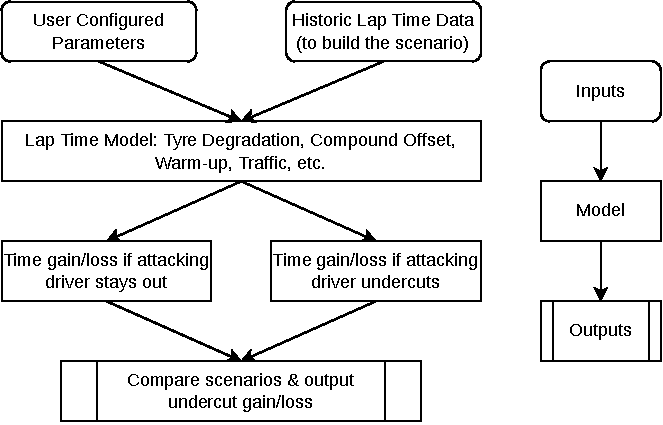
\includegraphics[width=\textwidth]{Figures/3_architecture_model.pdf}
    \caption{Information flow through the proposed undercut analysis model.}
    \label{fig:architecture-model}
\end{figure}

\section{Lap Time Model}
\label{sec:lap-time-model}

The scenario comparison requires a predicted lap time for each driver state.
The lap time model is therefore a supporting component rather than the sole
contribution of the dissertation. It is introduced in a deliberately simple
form before effects that require additional terms are added.

\subsection{Minimum Model}
\label{subsec:minimum-model}

The minimum model assumes that lap time $L$ is determined by reference pace
$B$, a compound offset $C$, and degradation loss $D(a)$ at tyre age $a$:

\begin{equation}
L=B+C+D(a).
\label{eq:minimum-lap-time}
\end{equation}
\myequation{Minimum lap time model}

Indices are intentionally omitted from \cref{eq:minimum-lap-time}. At this
stage they would add notation without improving the physical explanation. The
driver, scenario and lap indices are introduced only when the two futures are
accumulated in \cref{sec:cumulative-formulation}.

\subsubsection{Reference Pace}

The reference pace represents the underlying lap time of the selected driver
and car after the modelled tyre effects have been separated. When a common
event reference is used, an individual pace adjustment $P_d$ may be applied:

\begin{equation}
B_d=B_{\mathrm{ref}}+P_d.
\label{eq:driver-specific-ref-time}
\end{equation}
\myequation{Driver-specific reference pace}

% TODO: Choose one final estimation method. State the laps used, excluded lap
% types, fuel or track-evolution correction, and whether P_d is derived from
% historic data or supplied as an input. The method must prevent genuine
% driver/car pace from being misidentified as a tyre effect.

\subsubsection{Compound Offset}

The compound offset $C$ represents the lap time difference associated with a
tyre compound relative to a declared reference compound. As discussed in
\cref{subsec:tyre-compounds} and illustrated in
\cref{fig:1_conceptual_tyres}, the compounds provide different levels of grip
and durability. The offset is event-specific unless validation establishes
that a more general value is defensible.

% TODO: State how offsets are derived or supplied. Do not use generic fixed
% Soft/Medium/Hard values as evidence; label worked-example values as
% illustrative.

\subsubsection{Linear Degradation}

For the minimum model, degradation is approximated as a linear loss over the
short comparison window:

\begin{equation}
D(a)=ka,
\label{eq:linear-degradation}
\end{equation}

where $k$ is the degradation rate in seconds per lap of tyre age. Substitution
into \cref{eq:minimum-lap-time} gives

\begin{equation}
L=B+C+ka.
\label{eq:model-plus-tyre-degradation}
\end{equation}
\myequation{Minimum lap time model with linear degradation}

The approximation does not imply that an entire tyre stint is physically
linear. It provides an interpretable local model whose adequacy over the short
offset window can be tested against historic cases and through sensitivity
analysis.

% TODO: Define tyre age precisely. State whether age zero denotes an unused
% tyre before its out lap or the first completed timed lap. This convention is
% a likely source of off-by-one implementation errors.

\section{Progressive Model Extensions}
\label{sec:model-extensions}

Reference pace, compound offset and linear degradation specify terms already
present in the minimum model. The following additions are genuine extensions:
each introduces an effect that the minimum formulation cannot represent. For
every retained extension, document its engineering motivation, mathematical
form, parameter source and validation status.

\subsection{Tyre Warm Up Loss}
\label{subsec:warmup-model}

Freshly fitted tyres may not deliver their steady-state performance immediately.
A warm up term $W(i)$ is therefore added, where $i$ is the post-stop lap index:

\begin{equation}
L=B+C+D(a)+W(i).
\label{eq:model-plus-warmup}
\end{equation}
\myequation{Lap time model with tyre warm up loss}

% TODO: Select and justify the implemented form of W(i). If the software uses
% one out-lap penalty, state that directly. Do not imply a thermal tyre model.

\subsection{Traffic and Rejoin Effects}
\label{subsec:traffic-model}

An early stop can cause the attacking driver to rejoin behind slower traffic.
This changes the achievable lap time even when the fresh tyre advantage is
large. A traffic or rejoin penalty $R(i)$ extends the model to

\begin{equation}
L=B+C+D(a)+W(i)+R(i).
\label{eq:model-plus-traffic}
\end{equation}
\myequation{Lap time model with warm up and traffic effects}

Rejoin feasibility and time loss are related but distinct. Pit lane loss and
the current race gaps determine where the car rejoins; $R(i)$ represents the
additional lap time consequence after it has rejoined.

% TODO: State whether R(i) is derived from historic positions and gaps, entered
% as a configurable penalty, or omitted from the validated model. Do not claim
% predictive traffic simulation unless it has been implemented and verified.

\subsection{Used Replacement Tyres}
\label{subsec:used-tyres}

A replacement set need not be new. A used set is represented by assigning a
non-zero initial tyre age in the undercut scenario. This changes the degradation
term without requiring another additive lap time component. Any interaction
with the selected warm up representation must be stated explicitly.

\subsection{Effects Outside the Retained Model}
\label{subsec:optional-effects}

% LOWER PRIORITY: discuss only effects relevant to the final implementation.
% Candidate omissions include fuel mass, track evolution, non-linear
% degradation, driver variability and stochastic race interruptions. Explain
% the capability each would add before proposing it as future work.

\section{Cumulative Scenario Formulation}
\label{sec:cumulative-formulation}

Once the lap time components have been established, indices are required to
distinguish driver $d$, scenario $s$ and lap $i$. The complete retained lap time
model is written as

\begin{equation}
L_{d,s}(i)=B_d+C_{c_{d,s,i}}+D_{c_{d,s,i}}(a_{d,s,i})
            +W_{c_{d,s,i}}(i)+R_d(i).
\label{eq:complete-lap-time-model}
\end{equation}
\myequation{Complete indexed lap time model}

% Remove terms from this equation if they are not present in the final tested
% implementation, or mark them explicitly as optional. The dissertation must
% describe the model actually evaluated rather than an aspirational model.

The cumulative predicted time for scenario $s$ over $n$ comparison laps is

\begin{equation}
T_s(n)=\sum_{i=1}^{n}L_{\mathrm{att},s}(i)+Q_s,
\label{eq:cumulative-scenario-time}
\end{equation}
\myequation{Cumulative scenario time}

where $Q_s$ contains only scenario-specific pit, in-lap, out-lap or rejoin
adjustments not already included in the lap predictions. Common terms must not
be counted twice. The predicted undercut gain is defined as

\begin{equation}
G(n)=T_{\mathrm{stay}}(n)-T_{\mathrm{undercut}}(n).
\label{eq:undercut-gain}
\end{equation}
\myequation{Predicted undercut gain}

Under this sign convention, $G(n)>0$ indicates that pitting at the decision
point is predicted to save time, while $G(n)<0$ indicates a predicted loss.
This convention must be used consistently in the software, plots and validation
results.

\section{Model Outputs and Decision Metrics}
\label{sec:model-outputs}

The cumulative strategy gain $G(n)$ is the primary engineering output. Applying
that gain to the observed pre-decision gap produces a predicted post-stop gap
to the target driver. A track-position indicator can then report whether the
predicted gap crosses zero, while retaining the underlying continuous result
for interpretation and sensitivity analysis.

% TODO: Define the initial-gap sign convention and give the exact post-stop-gap
% equation. Also state whether the software reports the best tested offset,
% crossover lap, rejoin traffic warning, or any uncertainty interval.

\section{Definitions and Notation}
\label{subsec:notation}

Table \ref{tab:model_notation} consolidates the symbols introduced throughout
the model. A symbol is explained in detail when it first adds a capability; the
table then provides a single reference for its unit and scope.

\begin{table}[htbp]
\centering
\caption{Notation used throughout the proposed undercut model.}
\label{tab:model_notation}

\begin{tabular}{|l|l|p{7.5cm}|l|}
\hline
\textbf{Symbol} & \textbf{Unit} & \textbf{Definition} & \textbf{Scope} \\
\hline

$i$ & -- &
Lap index within the comparison window. &
$i = 1,2,\ldots,n$ \\
\hline

$n$ & laps &
Number of laps included in the comparison window. &
Scenario-independent \\
\hline

$a$ & laps &
Tyre age at the start of a lap. &
Driver-specific \\
\hline

$d$ & -- &
Driver identifier. &
Attacking or target driver \\
\hline

$c$ & -- &
Tyre compound identifier. &
Soft, Medium or Hard \\
\hline

$s$ & -- &
Strategy scenario. &
Undercut or Stay Out \\
\hline

$B_d$ & s &
Reference lap time of driver $d$, excluding tyre-related effects and configurable model adjustments. &
Driver \\
\hline

$P_d$ & s &
Pace adjustment of driver $d$ relative to the event reference pace. &
Driver \\
\hline

$C_c$ & s &
Lap time offset associated with tyre compound $c$. &
Compound \\
\hline

$D_c(a)$ & s &
Lap time loss due to tyre degradation as a function of tyre age. &
Compound, tyre age \\
\hline

$W_c(i)$ & s &
Warm-up penalty applied following a tyre change. &
Compound, lap \\
\hline

$R_d(i)$ & s &
Additional configurable lap time penalty due to traffic or other external effects. &
Driver, lap \\
\hline

$L_{d,s}(i)$ & s &
Predicted lap time of driver $d$ on lap $i$ under strategy scenario $s$. &
Driver, scenario, lap \\
\hline

$P$ & s &
Pit lane traversal and service loss common to equivalent stops. &
Pit stop \\
\hline

$Q_s$ & s &
Scenario-specific timing adjustments not already included in the predicted lap times. &
Scenario \\
\hline

$T_s(n)$ & s &
Cumulative predicted race time after $n$ comparison laps for strategy scenario $s$. &
Scenario \\
\hline

$G(n)$ & s &
Predicted undercut gain, defined as stay out scenario time minus undercut scenario time. &
Comparison window \\
\hline

\end{tabular}
\end{table}


\section{Model Parameters and Data Provenance}
\label{sec:model-parameters}

% VERY HIGH PRIORITY. Add one or more readable tables with:
% Parameter | Symbol | Unit | Scenario/driver | Source | Treatment.
% Separate measured historic fields, values derived from those fields, and
% configurable assumptions. Naming an API alone is not sufficient provenance.
% Resolve FastF1 versus OpenF1 consistently across Chapters 3--5, references,
% and the data/licensing appendix.
%
% Identify the baseline value and sensitivity range for every parameter tested
% in Chapters \ref{chap:validation-method} and \ref{chap:results}.

\section{Worked Numerical Example}
\label{sec:worked-example}

% HIGH VALUE. Add a deliberately simple fictional example containing:
% - the initial gap and both drivers' tyre states;
% - two or three offset laps;
% - the stay out and undercut lap predictions;
% - cumulative totals and common pit-loss cancellation;
% - G(n), the post-stop gap and the decision interpretation.
% Label every value as illustrative rather than validation evidence.

\section{Assumptions and Applicability}
\label{sec:model-assumptions}

% Add a table: Assumption | Rationale | Consequence | Tested/mitigated in.
% Include deterministic inputs, local linear degradation, short comparison
% window, equivalent pit losses, dry/green running, two-driver scope, baseline
% pace treatment, traffic representation and data completeness.
%
% An assumption defines model operation. A limitation is the resulting
% restriction on applicability or generalisability. Keep those ideas distinct.

\section{Chapter Summary}
\label{sec:model-summary}

% Summarise only the final retained model, output metrics and principal
% assumptions. Conclude by stating that Chapter \ref{chap:implementation}
% translates the methodology into software without changing its engineering
% logic.

\chapter{Model Implementation}
\label{chap:implementation}

% ============================================================================
% CHAPTER PURPOSE
% Explain how the Chapter \ref{chap:model} formulation was implemented as a
% reproducible analysis tool. Software engineering is relevant where it protects
% calculation correctness, traceability, experimentation or usability; avoid a
% generic catalogue of frameworks and coding practices.
% ============================================================================

\section{Implementation Requirements}
\label{sec:implementation-requirements}

% HIGH PRIORITY. Translate research objectives into functional requirements:
% - load/select historic meeting, session and drivers;
% - obtain/prepare lap, stint, compound and pit information;
% - configure assumptions/parameters;
% - execute both scenarios for candidate decision laps;
% - display numerical and race trace outputs;
% - retain enough metadata for reproduction.
% Add non-functional requirements only where relevant: determinism, separation
% of model/UI, responsiveness, offline analysis and clear error handling.

\section{Technology and Architecture Selection}
\label{sec:technology-selection}

\subsection{Initial Web-Based Approach}
% Briefly describe the original Blazor/client-server proposal and what research
% need it was intended to satisfy. Do not teach basic client-server architecture.
% The generic web architecture figure should be removed unless directly useful.

\subsection{Transition to WPF}
% Preserve the existing rationale but tighten it into an engineering decision:
% - limited project time and front-end experience;
% - unreliable debugging/development setup;
% - WPF enabled focus on model functionality and repeatable desktop analysis;
% - trade-off: Windows-only tool and reduced deployment flexibility.
% Avoid self-deprecating wording. Demonstrate risk management and scope control.

\subsection{Final Architecture}
% SUGGESTED FIGURE 4.1 -- MUST HAVE:
% Data provider -> preprocessing/domain data -> model engine -> result objects ->
% race trace/UI. Show where user parameters enter.
% Explain separation of model engine from presentation so equations can be unit
% tested and reused without the WPF UI.

\section{Historic Data Acquisition}
\label{sec:data-acquisition}

\subsection{Data-Source Evaluation}
% Clarify the final role of FastF1 and OpenF1. Earlier drafts mention moving from
% FastF1 to OpenF1, while appendices still list FastF1. Resolve this explicitly:
% - what each source was evaluated for;
% - which is used in the final implementation;
% - whether both are used for different responsibilities;
% - licensing, rate limits, availability and fields required.
% Cite official documentation/repositories and record exact versions/endpoints.

\subsection{Meeting, Session and Driver Selection}
% Explain mapping from championship/event/session to driver records.
% Include sprint/race session handling if implemented.
% LOW/MEDIUM PRIORITY screenshots can illustrate workflow, but avoid turning
% this into a user manual.

\subsection{Lap, Stint and Pit Stop Preparation}
% HIGH PRIORITY. Describe transformations that affect model validity:
% - invalid/incomplete laps;
% - pit in/out laps;
% - Safety Car/VSC filtering;
% - compound and tyre-age reconstruction;
% - missing sectors/lap times;
% - data ordering and synchronisation;
% - whether laps are fuel-corrected or left as observed.
% This is engineering methodology, not merely implementation detail.

\subsection{Caching and Reproducibility}
% MEDIUM PRIORITY. If API responses are cached/localised, explain how this
% protects reproducibility and avoids data changes/rate limits.
% Record session identifiers and parameter sets used in validation.

\section{Model Engine Implementation}
\label{sec:model-engine-implementation}

\subsection{Domain Representation}
% Explain the principal model entities conceptually: driver state, tyre state,
% scenario, lap prediction and comparison result. A small class/domain diagram
% is useful only if it clarifies correspondence with Chapter 3 notation.

\subsection{Scenario Calculation Workflow}
% Map implementation steps directly to equations/sections:
% 1. build decision state;
% 2. predict each scenario lap;
% 3. apply optional penalties;
% 4. accumulate to common endpoint;
% 5. generate gain/post stop metrics;
% 6. repeat across candidate laps/offsets.
% Include pseudocode or a flowchart rather than large C# listings.

\subsection{Parameter Configuration and Traceability}
% Explain how values are entered/derived and associated with a run.
% Show validation of units/ranges and handling of missing values.
% Consider a parameter-summary panel/export if implemented.

\subsection{Error Handling}
% MEDIUM PRIORITY. Cover only failures that affect engineering confidence:
% unavailable API, incomplete session, invalid tyre age, no comparison window,
% or impossible parameter values. State whether the user is warned or the case
% is excluded; never silently substitute unsupported data.

\section{Race Trace Visualisation}
\label{sec:race-trace}

\subsection{Race Trace Definition}
% Briefly explain axes/reference convention for a reader unfamiliar with race
% traces. State exactly how gap is calculated and what the reference line means.

\subsection{Opportunity and Event Annotations}
% VERY HIGH VALUE to practical contribution.
% Mark as applicable:
% - actual pit stops;
% - tyre compounds/stint boundaries;
% - model decision point;
% - predicted gain/crossover;
% - actual post stop outcome;
% - excluded/invalid periods.
%
% SUGGESTED FIGURES:
% 4.2 unannotated historic race trace;
% 4.3 same trace with model annotations and explanatory callouts.
% Use real application output when available, not only mock-ups.

\subsection{Interaction and Usability}
% MEDIUM PRIORITY. Briefly explain race/session loading, driver selection and
% parameter options. Tie usability to rapid engineering interrogation rather
% than claiming a full formal UX study unless one was conducted.

\section{Software Verification}
\label{sec:software-verification}

% HIGH PRIORITY but concise. This belongs here/methodology Chapter 5, not as a
% dominant research result.
% Explain the test layers planned/used:
% - unit tests for individual equations and sign conventions;
% - boundary tests for tyre age, zero degradation and zero offset;
% - integration tests from data state to scenario result;
% - regression tests for known parameter sets;
% - manual comparison with the Chapter 3 worked example.
% Report actual results in Chapter \ref{chap:results} or an appendix.

\section{Development Process and Key Iterations}
\label{sec:development-process}

% Retain the useful diary/sprint narrative from the earlier report, but make it
% analytical rather than chronological padding. For each significant iteration:
% - intended outcome;
% - problem discovered;
% - evidence/constraint;
% - decision made;
% - consequence for model/research scope.
% Include revised dates following the leave of absence.
% Candidates: data-source changes, Blazor->WPF, API reliability, race trace
% development and model iteration.
% Detailed sprint logs may go to an appendix; keep only consequential decisions
% in the chapter.

\section{Implementation Limitations}
\label{sec:implementation-limitations}

% Discuss software/data limitations separately from model limitations:
% - dependency on third-party historic data;
% - Windows/WPF platform restriction;
% - manual parameters;
% - incomplete data or API reliability;
% - no live operational integration.
% State consequence and mitigation. Do not repeat Chapter 6's engineering model
% limitations verbatim.

\section{Chapter Summary}
\label{sec:implementation-summary}

% One concise paragraph linking the implemented workflow to the verification and
% validation methodology in Chapter \ref{chap:validation-method}.

\chapter{Verification and Validation Methodology}
\label{chap:validation-method}

% ============================================================================
% CHAPTER PURPOSE -- VERY HIGH PRIORITY
% Define HOW correctness and credibility will be assessed. Keep results out of
% this chapter except for tiny illustrative checks. Chapter \ref{chap:results}
% reports outcomes.
%
% Distinguish terminology:
% - software verification: was the model implemented correctly?
% - model verification: do equations/logical behaviours behave as intended?
% - validation: does the model adequately represent observed race behaviour for
%   its stated purpose and operating domain?
% ============================================================================

\section{Evaluation Framework}
\label{sec:evaluation-framework}

% Introduce the chain of evidence:
% equation checks -> software tests -> limiting/expected-behaviour tests ->
% historic-case validation -> sensitivity/uncertainty analysis.
% SUGGESTED FIGURE 5.1: verification and validation workflow.
% Map each method to a success criterion from Section \ref{sec:success-criteria}.

\section{Software and Calculation Verification}
\label{sec:calculation-verification}

\subsection{Unit-Test Design}
% Define test families and expected values, not framework trivia:
% - base lap with all penalties zero;
% - tyre age/degradation increments;
% - compound offset;
% - warm-up only on intended laps;
% - cumulative summation;
% - sign convention for gain;
% - initial gap to post stop gap conversion;
% - common pit loss cancellation;
% - invalid/missing inputs.
% Put exhaustive test-case tables/screenshots in Appendix \ref{app:software-tests}.

\subsection{Integration and Regression Testing}
% Verify data ingestion -> model state -> result -> visual marker.
% Fix at least one known scenario/parameter set as a regression case.
% State pass/fail criteria before reporting results.

\subsection{Independent Hand Calculation}
% HIGH VALUE. Recalculate the worked example independently (spreadsheet/manual)
% and compare it with software output. This is stronger evidence than tests that
% reproduce the same implementation logic.

\section{Model Behaviour Verification}
\label{sec:model-behaviour-verification}

% Test limiting and monotonic behaviours expected from the formulation:
% - zero degradation and equal compounds -> near-zero tyre-driven gain;
% - increased target degradation -> stronger undercut, all else equal;
% - larger warm-up penalty -> weaker undercut;
% - traffic penalty -> weaker undercut;
% - zero offset laps -> no offset-lap gain;
% - identical scenarios -> zero gain;
% - used replacement tyre behaves consistently with starting age.
% These tests answer "does the model make engineering sense?" before historic
% validation.

\section{Historic Validation Case Selection}
\label{sec:case-selection}

% VERY HIGH PRIORITY. Define transparent selection criteria to avoid cherry
% picking. Aim for a small but varied set rather than one famous success.
% Candidate categories:
% - clear successful undercut;
% - unsuccessful/neutral attempt;
% - case compromised by traffic/warm-up;
% - different circuits/compounds/offset lengths;
% - optional negative-control period with no expected opportunity.
% Explain data completeness and why the cases are observable.
% Record excluded cases and reasons in Appendix \ref{app:validation-data}.

\section{Historic Data Preparation}
\label{sec:validation-data-prep}

% Define consistently:
% - decision lap and common comparison endpoint;
% - actual tyre ages/compounds;
% - treatment of in/out laps;
% - removal/retention of laps affected by flags, traffic or errors;
% - base pace and degradation estimation method;
% - parameter values unavailable directly from data;
% - actual observed gain metric.
% This section is crucial for reproducibility and prevents hindsight bias.

\section{Validation Metrics}
\label{sec:validation-metrics}

% Define metrics before seeing/reporting conclusions. Possible metrics:
% - predicted and observed gain in seconds;
% - signed error e = predicted - observed;
% - absolute error;
% - correct direction/classification of gain/loss;
% - post stop gap error;
% - opportunity-lap timing error if detecting a window.
% For a small sample, do not overstate statistical power. Report each case and
% summary statistics transparently.

\section{Sensitivity Analysis Method}
\label{sec:sensitivity-method}

% VERY HIGH PRIORITY / likely major mark source.
% Establish:
% - baseline case/parameter set;
% - parameter ranges and justification;
% - one-at-a-time (OAT) method for interpretability;
% - optional multi-parameter scenarios/interactions if time permits;
% - output metric (usually change in G or threshold/crossover).
% Minimum parameters:
% - degradation rate/current tyre age;
% - compound offset;
% - replacement tyre warm-up;
% - number of offset laps;
% - relative driver/car base pace;
% - traffic penalty if retained.
% Pit loss should be treated with the symmetry discussion from Section
% \ref{sec:pit-loss}; test unequal/rejoin effects only if relevant.
%
% MEDIUM/LOW PRIORITY extension:
% factorial/global sensitivity or Monte Carlo uncertainty. Do not add this at
% the expense of a complete, well-explained OAT analysis.

\section{Uncertainty and Error Treatment}
\label{sec:uncertainty-method}

% HIGH VALUE. Identify uncertainty sources:
% - noisy/traffic-affected historic lap times;
% - degradation fit uncertainty;
% - unknown warm-up/traffic penalty;
% - driver/car pace changes;
% - API missing/incorrect fields.
% State whether uncertainty is represented by ranges, alternate assumptions,
% confidence intervals, or qualitative caveats.
% Avoid claiming precise predictive certainty from manually selected inputs.

\section{Validation Threats and Bias Control}
\label{sec:validation-threats}

% MEDIUM/HIGH VALUE.
% Address:
% - hindsight in selecting known undercuts;
% - circularity if parameters are fitted using the same outcome being predicted;
% - confounding from driver pace, fuel, traffic and track evolution;
% - small case count/generalisation;
% - data-source limitations.
% Explain mitigations such as fixed selection criteria, holdout cases, baseline
% extraction before examining the outcome, and reporting failed cases.

\section{Software Usability Check}
\label{sec:usability-check}

% LOW PRIORITY. Only include if actually done.
% A short task-based check can confirm that a user can load a race, configure a
% scenario and interpret an annotation. Do not imply formal human-subject UX
% research without appropriate design/ethics.

\section{Chapter Summary}
\label{sec:validation-method-summary}

% Summarise the evidence that will be reported in Chapter \ref{chap:results}.

\chapter{Results and Evaluation}
\label{chap:results}

% ============================================================================
% CHAPTER PURPOSE -- VERY HIGH PRIORITY
% Present evidence generated by Chapter \ref{chap:validation-method}, interpret
% it and answer the research questions. Separate observed result from
% explanation. Do not repeat methodology at length.
% ============================================================================

\section{Implementation and Verification Results}
\label{sec:verification-results}

\subsection{Software Test Results}
% Concise summary table: test family | count | result | notable issue.
% Detailed test cases belong in Appendix \ref{app:software-tests}.
% Report failures and corrections honestly; a defect found and fixed is useful
% verification evidence.

\subsection{Hand-Calculation Comparison}
% Present software versus independent calculation and numerical difference.
% Explain any rounding/indexing convention.

\subsection{Expected-Behaviour Results}
% Table/plots for limiting cases from Section
% \ref{sec:model-behaviour-verification}. Interpret whether the direction and
% magnitude are consistent with the equations and strategy reasoning.

\section{Historic Case Results}
\label{sec:historic-results}

% Use a consistent repeated structure for each case rather than free-form prose.
% For each:
% 1. race context and why selected;
% 2. decision state and input table;
% 3. predicted gain/post stop outcome;
% 4. actual observed result;
% 5. error and explanation;
% 6. annotated race trace.

\subsection{Successful Undercut Case(s)}
% HIGH PRIORITY. Include at least one clear success, but do not rely only on
% successes.

\subsection{Unsuccessful or Neutral Case(s)}
% HIGH PRIORITY. Demonstrating a negative prediction/outcome materially improves
% credibility and allows failure conditions to be discussed.

\subsection{Compromised or Boundary Case(s)}
% MEDIUM/HIGH PRIORITY. Traffic, warm-up, low degradation or unusual pace.
% Useful for showing limits of the minimum model and value of extensions.

\subsection{Cross-Case Validation Summary}
% MUST-HAVE TABLE:
% Case | predicted gain | observed gain | signed/absolute error | direction
% correct? | key confounder.
% Report aggregate values cautiously due to likely small sample size.

\section{Sensitivity Analysis Results}
\label{sec:sensitivity-results}

% VERY HIGH PRIORITY. Use a baseline case and one clear graph per parameter or a
% well-designed combined summary. Every graph requires:
% - baseline and range;
% - trend/threshold;
% - engineering explanation;
% - implication for strategy/model use.

\subsection{Tyre Degradation and Tyre Age}
% Examine both rate and current age where distinguishable.
% Identify threshold at which predicted gain changes sign if present.

\subsection{Compound Performance Delta}
% Explain interaction with offset length and warm-up.

\subsection{Offset-Lap Count / Target Stop Timing}
% This is likely a dominant mechanism; show cumulative nature clearly.

\subsection{Warm-Up Loss}
% Compare no warm-up, baseline and adverse warm-up assumptions.

\subsection{Relative Driver/Car Pace}
% HIGH PRIORITY to prevent strategy gain being mistaken for underlying pace.

\subsection{Traffic / Rejoin Penalty}
% Include if the term is retained in the final model.

\subsection{Sensitivity Ranking and Interactions}
% Summarise normalised/representative impact in a tornado/ranked table.
% MEDIUM PRIORITY: show one or two meaningful parameter interactions, such as
% degradation x warm-up or offset laps x compound delta. Do not create an
% exhaustive design if time is limited.

\section{Research Question Evaluation}
\label{sec:rq-evaluation}

% Answer each research question explicitly, with evidence citations to the
% relevant table/figure. Distinguish "supported for selected cases" from broad
% universal claims.

\section{Engineering Discussion}
\label{sec:engineering-discussion}

\subsection{Conditions Favouring an Undercut}
% Synthesise results: fresh-tyre delta, target degradation, offset duration,
% warm-up, clear rejoin and relative pace. Avoid simply restating graph slopes.

\subsection{Conditions Favouring Staying Out or an Overcut}
% Use negative/weak undercut results to explain low degradation, adverse warm-up,
% traffic and strong old-tyre pace. This demonstrates system understanding even
% if overcut is not fully implemented.

\subsection{Practical Interpretation of Model Output}
% Explain how an engineer should use G, post stop gap and race trace annotation:
% as decision support subject to assumptions, not an autonomous instruction.
% Discuss required margin when inputs are uncertain.

\subsection{Comparison with Existing Research}
% Return to Chapter \ref{chap:background}: where do observed trends agree or
% disagree with literature/accepted strategy mechanisms? Explain differences.

\section{Model Validity, Limitations and Generalisability}
\label{sec:validity-limitations}

% Organise rather than repeat a generic limitation list:
% - internal validity: implementation and parameter fitting;
% - construct validity: whether G captures "undercut effectiveness";
% - external validity: circuits/races/conditions beyond tested cases;
% - data limitations;
% - omitted dynamics and uncertainty.
% State which findings are robust and which are conditional.

\section{Objective Achievement Summary}
\label{sec:objective-achievement-results}

% Concise table: objective | evidence | status | caveat.
% This creates a direct bridge to Chapter \ref{chap:conclusion}.

\section{Chapter Summary}
\label{sec:results-summary}

% 1--2 paragraphs containing only the principal evidence-based findings.
% Do not introduce future work here; reserve it for Chapter 7.

\chapter{Conclusion and Future Work}
\label{chap:conclusion}

% ============================================================================
% CHAPTER PURPOSE
% Close the argument. Do not introduce new evidence, equations or literature.
% Keep this chapter comparatively short and decisive.
% ============================================================================

\section{Research Aim and Approach}
\label{sec:conclusion-aim}

% Restate the aim in past tense and summarise the approach in 1--2 paragraphs:
% transparent deterministic model, software implementation, historic validation
% and sensitivity analysis. Do not repeat chapter-by-chapter contents.

\section{Principal Findings}
\label{sec:principal-findings}

% VERY HIGH PRIORITY. State only findings supported by Chapter 6, ideally in
% order of the research questions:
% - level of agreement with historic cases;
% - dominant parameters/mechanisms;
% - conditions under which predictions became unreliable;
% - value/limitations of race trace interpretation.
% Include numbers where they are the clearest summary, but no new tables.

\section{Achievement of Objectives}
\label{sec:objective-achievement-conclusion}

% Briefly revisit each numbered objective from Section
% \ref{sec:research-objectives}. Avoid duplicating the detailed Chapter 6 table;
% synthesise what was fully achieved, partially achieved or excluded.

\section{Contributions}
\label{sec:contributions}

% Be accurate and proportionate; "contribution" does not require claiming a new
% universal theory.
%
% Methodological/engineering contributions may include:
% - transparent decomposition of undercut gain into auditable components;
% - explicit treatment of common pit-loss cancellation;
% - progressive minimum-to-extended model and evaluation method;
% - evidence about parameter sensitivity for the selected cases.
%
% Practical contributions may include:
% - working historic-analysis application;
% - annotated race trace linking prediction and actual outcome;
% - reusable parameterised workflow.
% Only claim items actually delivered and evaluated.

\section{Recommendations for Use}
\label{sec:recommendations}

% MEDIUM PRIORITY but valuable.
% State the operating conditions in which the model is most defensible and the
% checks a user should perform before acting on its result. Emphasise decision
% support and safety margin under uncertain inputs.

\section{Future Work}
\label{sec:future-work}

% Prioritise extensions by the limitation they address and expected value.
% Suggested order:
% 1. improve degradation estimation/non-linear or stint-specific fitting;
% 2. quantify uncertainty and produce prediction ranges;
% 3. dynamic rejoin/traffic and multi-car interaction;
% 4. model overcut explicitly using the same comparative framework;
% 5. Safety Car/VSC/weather/probabilistic whole-race simulation;
% 6. live timing integration and prospective validation.
% For each: limitation -> proposed method -> expected benefit.
% Avoid a disconnected wish list (especially "use AI/ML" without justification).

\section{Final Statement}
\label{sec:final-statement}

% One concise closing paragraph that answers the original aim and leaves a
% balanced statement of usefulness and limits.

% add any additional chapters here

%TC:ignore
\setemptyheader

\nocite{*} % include everything from the bibliography, irrespective of whether it has been referenced.

% the following line is included so that the bibliography is also shown in the table of contents. There is the possibility that this is added to the previous page for the bibliography. To address this, a newline is added so that it appears on the first page for the bibliography. 
%\addcontentsline{toc}{chapter}{Bibliography} % Adds References to contents page

%
% example of including an annotated bibliography. The current style is an author date one. If you want to change, comment out the line and uncomment the subsequent line. You should also modify the packages included at the top (see the notes earlier in the file) and then trash your aux files and re-run. 
%\bibliographystyle{StylesAndReferences/authordate2annot}
\bibliographystyle{StylesAndReferences/IEEEannotU}
\bibliography{StylesAndReferences/references} % References file

\cleardoublepage
\phantomsection
\chapter*{Selected Background Reading}
\addcontentsline{toc}{chapter}{Selected Background Reading}

[x - any bibliography books]

\begin{description}

\item[Milliken \& Milliken (1995)]
Race Car Vehicle Dynamics.
SAE International.

\item[Bentley (2011)]
Ultimate Speed Secrets.
Motorbooks.

\item[Smith (1996)]
Drive to Win.
Aero Publishers.

\end{description}

\setemptyheader

\addcontentsline{toc}{chapter}{Appendices}
\pagebreak

% start the appendix - sets up different numbering
\fancypagestyle{plain}{%
%\fancyhf{} % clear all header and footer fields
\fancyhead[L]{Appendix\ \thechapter}
\fancyhead[R]{\leftmark}}

\appendix
\fancyhead[L]{Appendix\ \thechapter}
\fancyhead[R]{\leftmark}
\fancyhead[C]{}
\fancyfoot[C]{\thepage}
\renewcommand{\headrulewidth}{0.4pt}
\renewcommand{\chaptermark}[1]{\markboth{#1}{}}

\fancyhead[L]{Appendix\ \thechapter}
\fancyhead[R]{\leftmark}
\fancyfoot[C]{{\thepage} of \pageref{LastPage}}

\renewcommand{\thesection}{\thechapter.\arabic{section}}

% include any appendices here
\chapter{Glossary}
\addcontentsline{toc}{chapter}{Glossary}

\begin{center}
\begin{tabular}{p{0.2\textwidth}p{0.7\textwidth}}
\textbf{Term} & \textbf{Explanation} \\ \hline
Marbles & [x] \\
In \& Out Lap & [x] \\
Undercut & [x] \\
Overcut & [x] \\
\end{tabular}
\end{center}
\chapter{Third-Party Code and Libraries}

\begin{itemize}
    \item FastF1 - [x - Description of the tool.][x - Version used]. The library is open source, available for download using 'pip' or cloned from GitHub \cite{software_fastf1}. This library is released using the MIT License \cite{license_mit}. This library was used without modification.
\end{itemize}
\chapter{Version History}

\begin{table}[h]
\centering
\begin{tabularx}{\textwidth}{|c|c|X|}
\hline
\textbf{Version} & \textbf{Type} & \textbf{Changes} \\
\hline
0.1 & Draft & Initial Creation \\
\hline
1.0 & Release & Initial Release \\
\hline
\end{tabularx}%
\caption{Version History}
\label{my-label}
\end{table}
\include{Appendices/appendixD}
\include{Appendices/appendixE}
\include{Appendices/appendixF}

\fancypagestyle{plain}{%
   \fancyhead{} %[C]{Annotated Bibliography}
   \fancyfoot[C]{{\thepage} of \pageref{LastPage}} % except the center
   \renewcommand{\headrulewidth}{0pt}
   \renewcommand{\footrulewidth}{0pt}
}

%TC:endignore

\end{document}
